


\chapter[Analytical R-matrix theory]{Analytical $R$-matrix theory}
\label{chap:R-matrix}

In this chapter we lay the groundwork of the Analytical $R$-Matrix(ARM) theory of photoionization that we will use throughout Part~\ref{part:I} of this thesis, following the original presentation of the theory~\cite{ARM_initial, ARM_initial_multielectron} and the formulation in the author's MRes report~\cite{MResReport}; for a more compact presentation we refer the reader to Refs.~\citealp{Pisanty_slalom_2016} and~\citealp{ARM_abinitio_verification}. We present the basic framework in section~\ref{sec:basic-framework}, and then specialize this to the single-electron case in section~\ref{sec:direct-ionization-amplitude}, and we develop the multi-electron formalism further in section~\ref{sec:correlation-driven-ionization}. We also present, in section~\ref{sec:molecular-shape-factors}, original results for the ARM shape factor of molecules, obtaining simple analytical formulas for model asymptotic molecular orbitals.


The core of the $R$-Matrix method is the separation of space into an inner region and an outer one by a spherical boundary, which enables one to apply, in the two different regions, different methods and approximations, where they are relevant. In general, this is often done when there is a complex many-body system which is, nevertheless, well approximated as a single-particle problem outside of the given region.

The $R$-matrix method was developed by Wigner~\cite{Rmatrix_Wigner} as a technique to describe nuclear reactions~\cite{Rmatrix_nuclear_review}, and it was adapted in atomic physics to deal with collisions of slow electrons with atoms~\cite{Rmatrix_atomic} and molecules~\cite{Rmatrix_molecular}. In a strong-field context, the $R$-matrix as a numerical method permits a fuller description of multi-electron effects inside the molecule~\cite{ Rmatrix_time_dependent}, while at the same time handling strong-field phenomena whose large grids prevent the use of multiple electrons in the outer region.

$\quad$

\begin{figure}[b]
  \centering
  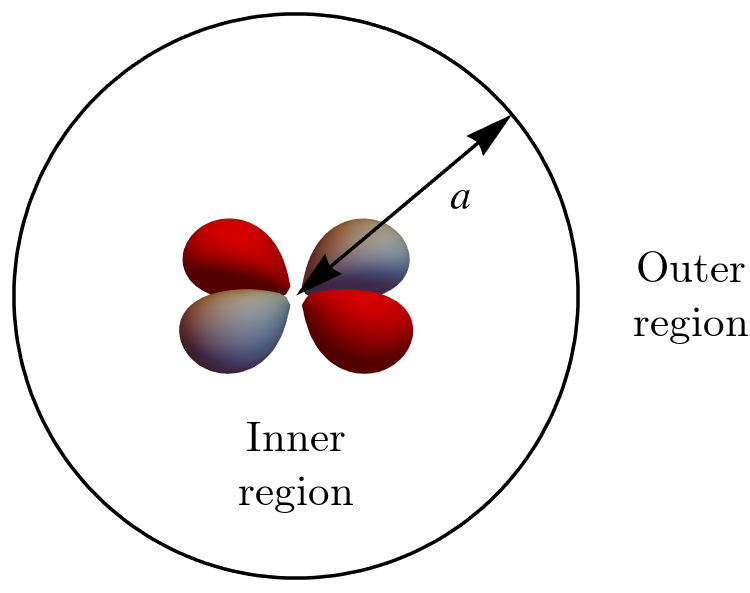
\includegraphics[scale=1]{2-ARM-theory/Figures/figure2E.png}
  \caption[$R$-matrix splitting of space]{$R$-matrix splitting of space into an inner spherical region of radius $a$ and an outer region outside that sphere.}
  \label{fig:2A-splitting-space}
\end{figure}

The Analytical $R$-Matrix method makes use of this spatial separation, not to implement different numerical methods on the two different regions, but rather to use different approximate analytical methods in their regions of validity. In particular, the solutions of the Schrödinger equation driven by the laser field -- the Volkov states we visited in the Introduction -- can be augmented to include the effect of the interaction with the parent ion through the eikonal-Volkov approximation~\cite{eikonalVolkov_initial, eikonalVolkov_prelim}, but this breaks down near the ion, so that solution needs to be fenced off from its singularities, where the normal atomic or molecular eigenstates can be used. Having done this, multi-electronic effects can then be built in by taking a single electron to be in the outer region and using the eigenstates of the ion as a basis, to which the outer electron is correlated.





In this chapter, we will show how these tools are built and come together to produce the theory: the separation of space, the different ingredient solutions, their integration, the encapsulation of the effect of the inner wavefunction on the outer one, and the use of the saddle-point approximation to produce clear physical pictures for the process.





\section{Basic framework}
\label{sec:basic-framework}

\subsection{Splitting space}


The separation of space into two parts, while conceptually simple, does pose some technical challenges that need to be addressed with the right language. Naively, we have an initial Hilbert space which describes wavefunctions over the whole of space,
\begin{equation}
\hil=\{\psi:\mathbb R^3\to \mathbb C \mid \int|\psi(\vbr)|^2 \d\vbr < \infty \}
\end{equation}
%
\begin{subequations}
%
and we want to separate it into functions from inside and outside the ball $B(a)$ of radius~$a$, 
\begin{align}
\hil_< & =\{\psi:B(a)\to \mathbb C \mid \int|\psi(\vbr)|^2 \d\vbr < \infty \} \\
\hil_> & =\{\psi:\mathbb R^3\setminus B(a)\to \mathbb C \mid \int|\psi(\vbr)|^2 \d\vbr < \infty \},
\end{align}
%
\end{subequations}
%
using the projectors $\Pi_\lessgtr:\hil \to \hil_\lessgtr$. We want to deal with the projected wavefunctions $\,\Pi_\lessgtr\! \ket\psi$ separately, so we simply project the Schrödinger equation as $i\frac{\d}{\d t} \,\Pi_\lessgtr\! \ket\psi=\,\Pi_\lessgtr  H \ket\psi$, and we reformulate it in terms of the projected wavefunctions. 

The technique is most easily illustrated, for simplicity, in one dimension (though of course it extends directly to the radius in three dimensions. Concentrating for the moment on the outer region, we're interested in the evolution of $\Pi_>\ket{\psi}$, which is given by
\begin{equation}
i\frac{\d}{\d t}\Pi_>\ket{\psi} 
= \Pi_> \,H\! \ket{\psi}
= H \,\Pi_> \!\ket{\psi} + \left[\Pi_>, \tfrac12\hat{p}^2\right]\ket{\psi},
\end{equation}
since the kinetic energy $\tfrac12\hat{p}^2$ does not commute with the spatial projection. To find the commutator $\left[\Pi_>, \tfrac12\hat{p}^2\right]$ that appears in the time evolution, the quickest route is to set $\Pi_> = \theta(\hat x-a)$, and to use the canonical commutation relation in the form
\begin{equation}
\hat{p} f(\hat{x}) = f(\hat{x}) \hat{p} -i f'(\hat{x}).
\end{equation}

Thus, we look at
\begin{align}
\hat{p}^2 \theta(\hat{x}-a)
& = 
\hat{p} \left( \theta(\hat{x}-a) \hat{p} - i \theta'(\hat{x}-a)\right)
\nonumber \\ & =
 -i\hat{p}\delta(\hat{x}-a)
 + \left(\theta(\hat{x}-a) \hat{p} - i \theta'(\hat{x}-a)\right)\hat{p}
\nonumber \\ & =
 -\left(i\hat{p}\delta(\hat{x}-a) + \delta(\hat{x}-a)i\hat{p} \right) 
 + \theta(\hat{x}-a)\hat{p}^2,
\end{align}
which then gives us the commutator as
\begin{equation}
\left[ \theta(\hat{x}-a),\hat{p}^2\right] = i\hat{p}\delta(\hat{x}-a) + \delta(\hat{x}-a)i\hat{p},
\end{equation}
and which we encapsulate using the notation
\begin{equation}
\hat{L}_0 \colonequals
\left[ \theta(\hat{x}-a),\tfrac12\hat{p}^2\right] = \frac{ i\hat{p}\delta(\hat{x}-a) + \delta(\hat{x}-a)i\hat{p}}{2},
\end{equation}
which is known as the Bloch operator, after Claude Bloch~\cite{ Bloch_L_operator_1957}.


With this commutator ready, the Schrödinger equation for the outside component~reads
\begin{equation}
i\frac{\d}{\d t} \theta(\hat{x}-a) \ket{\psi} 
= H \theta(\hat{x}-a)\ket{\psi} + \hat{L}_0\ket{\psi},
\end{equation}
%
\begin{subequations}
%
which we can further split into
\begin{equation}
i\frac{\d}{\d t} \theta(\hat{x}-a) \ket{\psi} 
= \left[ H + \hat{L}_0 \right] \theta(\hat{x}-a)\ket{\psi} + \hat{L}_0\theta(a-\hat{x})\ket{\psi}.
\end{equation}
Similarly, there is an identical equation for the inner wavefunction,
\begin{equation}
i\frac{\d}{\d t} \theta(a-\hat{x}) \ket{\psi} 
= \left[ H - \hat{L}_0 \right] \theta(a-\hat{x})\ket{\psi} - \hat{L}_0\theta(\hat{x}-a)\ket{\psi},
\end{equation}
%
\end{subequations}
%
and the two make up a pair of coupled inhomogeneous Schrödinger equations: each is governed by its own hamiltonian, altered with the addition of a Bloch operator to keep the per-component hamiltonian hermitian, and with coupled source terms $\pm\hat{L}_0 \theta(\mp(\hat{x}-a))\ket{\psi}$ that give the flow of probability from either region into the other.

In general, the coupled Schrödinger equations for the inner and outer regions are usually fine-tuned by the addition of a separate hermitian factor, to make the full Bloch operator read
\begin{equation}
L^{(\pm)}(a) = \pm \hat{L}_0 \pm \delta(\hat{x}-a)b(\hat{x}).
\label{e2-bloch-operator-with-function}
\end{equation}
%
\begin{subequations}
%
Ultimately we will choose $b(r) = (1-b)/r$, where $b$ is a constant, as it will significantly simplify the algebra, but for now we leave it arbitrary, and obtain our coupled Schrödinger equations in useful form:
\begin{empheq}[left=\empheqlbrace]{align}
i\frac{\d}{\d t}\ket{\psi_>} 
&= \left[ H - L^{(-)}(a) \right] \ket{\psi_>} - L^{(-)}(a) \ket{\psi_<},
\\
i\frac{\d}{\d t}\ket{\psi_<} 
&= \left[ H  - L^{(+)}(a) \right] \ket{\psi_<} - L^{(+)}(a)\ket{\psi_>}.
\end{empheq}
\end{subequations}


When solving these equations numerically, one usually keeps close track of both hamiltonians and both flow operators, and indeed in principle one can implement a full recollision step in ARM theory by using the in-flow from the outer region into the inner one, though this is as yet unexplored. For our purposes, however, it will be sufficient to look at the evolution of the outer region, and keep the inner-region wavefunction at the ground state of the neutral, essentially unperturbed, so $\ket{\psi_<}\approx \ket{\Psi_g}$, and this will work as our source term for the outer region.


We arrive, then, at the problem to be solved:
\begin{subequations}
\label{e2-problem}
\begin{align}
i\frac{\d}{\d t}\ket{\Psi(t)}
&=\left[H - \hat{L}^{(-)}(a)\right]\ket{\Psi(t)} -\hat{L}^{(-)}(a)\ket{\Psi_g}\!,
\\
\ket{\Psi(0)}&=\ket{\Psi_g}.
\end{align}
\end{subequations}
This problem can be solved formally, if one has access to the full propagator $U(t,t')$ corresponding to the $N$-electron hamiltonian $H$, satisfying $i\partial_t U(t,t') = H(t) U(t,t')$ under $U(t',t')=\id$, in which case the solution obeys
\begin{equation}
\ket{\Psi(t)}=-i\int_{-\infty}^t \!\d t' \, U(t,t')\hat{L}^{(-)}(a)\ket{\Psi_g(t')}.
\label{e2-formal-solution}
\end{equation}
Here we will take the state $\ket{\Psi(t)}$ inside the integral to be the neutral's ground state $\ket{\Psi_g}$, with ionization potential $I_p$ and energy $E_g=-I_p$: $\ket{\Psi_g(t)}= e^{+iI_p t}\ket{\Psi_g}$. This is the solution of the Schrödinger equation for the inner region obtained by ignoring backflow from the outer region and polarization of the neutral by the laser field; both of these effects can be reinstated later if required. As such, equation~\eqref{e2-formal-solution} represents a concrete Ansatz for the wavefunction we are looking for, and the problem now becomes that of obtaining suitable approximations for the propagator $U(t,t')$.




\subsection{The hamiltonian}
We wish to consider ionization of an atom or molecule by a strong, long-wavelength laser field, and we want to consider multi-electron effects. As such, the hamiltonian for the problem includes electrostatic forces for $N$ electrons, with nuclei of charge $Z_m$ at $\vb R_m$, and their length-gauge interaction with an external laser field~$\vb F(t)$:
\begin{subequations}
\label{e2-totalhamiltonian}
\begin{align}
H^N&=T_e^N+V_C^N+V_{ee}^N+V_L^N,\textrm{ where}\\
V_C^N&=-\sum_m \sum_{i=1}^N \frac{Z_m}{\|\vb{R}_m-\vb{r}_i\|},\\
V_{ee}^N&=\sum_{i>j}^N \frac{1}{\|\vbr_i-\vbr_j\|},\label{e2-V-ee-definition}\\
V_L^N&=\sum_{i=1}^N \vbf(t)\cdot \vbr_i.
\end{align}
\end{subequations}

Once the ionized electron leaves the molecule, the total hamiltonian is split into the $N-1$-electron ionic hamiltonian $H^{N-1}$, formally identical to the neutral one, and the hamiltonian for the leaving electron,
\begin{equation}
H_e\colonequals H^N-H^{N-1}
\end{equation}
which in particular contains the entangling operator $V_{ee}=V_{ee}^N-V_{ee}^{N-1}=\sum_{i=1}^{N-1}\|\vbr_i-\vbr\|^{-1}$, the Coulomb repulsion between the leaving electron and the ion. 

This hamiltonian can therefore be split into three specific components: the ionic core electrons in the inner region and their polarization by the laser field, the ionized electron and its strong driving in the outer region by the laser field, and their entangling interaction. We will add the entangling interaction in perturbatively, after developing approximate analytical propagators for each factor.



\subsection{Eikonal-Volkov states}
We begin by focusing on the ionized electron, which will be driven by a hamiltonian of the form
\begin{equation}
H_e=\frac12 \hat{\vbp}^2 + \vbf(t)\cdot\hat\vbr + V(\vbr),
\label{e2-single-electron-hamiltonian}
\end{equation}
where $V(\vbr)$ is an electrostatic interaction with the ionic core, and which is considered weak in the outer region. If one ignores this electrostatic interaction, leaving the laser-driven hamiltonian $H_L=\frac12 \hat{\vbp}^2 + \vbf(t)\cdot \hat\vbr$, the Schrödinger equation has well-known exact solutions known as Volkov states~\cite{ bergou_volkov_sates_1980}, as we met them earlier in \eqref{e1-volkov-wavefunctions},
\begin{align}
\phantom{{}^\mathrm{EA}}
\braket{\vb{r}}{\vb{k}^{\mathrm{(V)}}(t)}
& = 
\frac{1}{(2\pi)^{3/2}}
e^{i\left(\vb{k}+\vba(t)\right)\cdot\vb{r}} 
e^{-\frac{i}{2} \int_T^t\left(\vb{k}+\vba(\tau)\right)^2\d\tau},
\phantom{e^{-i\int_T^t U_n(\rl(\tau;\vb{r},\vb{k},t),\tau)\d\tau}}
\label{e2-volkov-wavefunctions}
\end{align}
defined in terms of the vector potential of the field $\vba(t)$, which must obey $\vbf(t) = -\frac{\d\vba}{\d t}$.

To include the interaction with the electrostatic potential $V(\vbr)$, we use the eikonal-Volkov approximation~\cite{eikonalVolkov_initial, eikonalVolkov_prelim}, which is an adaptation of the Wentzel-Kramers-Brillouin (WKB) method to the $V(\vbr)$-driven interaction-picture Schrödinger equation on top of the Volkov states of \eqref{e2-volkov-wavefunctions}: one posits a wavefunction modified by an amplitude and a phase, and then solves perturbatively for both. The result are the wavefunctions
\begin{align}
\braket{\vb{r}}{\vb{k}^{\mathrm{(EVA)}}(t)}
& = 
\frac{1}{(2\pi)^{3/2}}
e^{i\left(\vb{k}+\vba(t)\right)\cdot\vb{r}} 
e^{-\frac{i}{2} \int_T^t\left(\vb{k}+\vba(\tau)\right)^2\d\tau} 
e^{-i\int_T^t V(\rl(\tau;\vb{r},\vb{k},t),\tau)\d\tau},
\label{e2-eikonal-volkov-wavefunctions}
\end{align}
with an added Coulomb phase $e^{-iW_C}=e^{-i\int_T^t V(\rl(\tau;\vb{r},\vb{k},t),\tau) \d\tau}$ in terms of the laser-driven trajectory
\begin{align}
\rl(\tau;\vb{r},\vb{k},t)
& \colonequals 
\vb{r}+\int_t^\tau \left[\vb{k}+\vba(\tau')\right]\d\tau'
\label{e2-trajectory}
\end{align}
that starts at position $\vbr$ at time $t$ and has asymptotic momentum $\vbk$. The eikonal-Volkov states are in general valid as long as the boundary radius $a$ is far enough from the ion.






\subsection{Ionic states}
In addition to the continuum wavefunctions, in going from a single-active-electron approach to a multi-channel one where the ionized electron is entangled with the ionic core, we also require an appropriate basis of solutions for the different channels of the core. In particular, we want to solve the time-dependent Schrödinger equation in the inner region for the $N-1$ electrons of the ion, $i\partial_t\!\ket*{\Psi^{N-1}}=H^{N-1}\ket*{\Psi^{N-1}}$, potentially including polarization effects induced by the external field.

To solve this problem, we choose the basis of instantaneous eigenstates of the ion, which obey
\begin{equation}
H^{N-1}(t)\ket{n(t)}=E_n(t)\ket{n(t)}
\label{e2-quasistatic-eigenstates}
\end{equation}
at each instant $t$, and from which one can construct approximate TDSE solutions of the form 
$e^{-i\int^tE_n(\tau)\d \tau}\ket{n(t)}$ as long as the laser frequency $\omega$ is smaller than the characteristic energy spacing $\Delta E$ of the system.

In practice, this thesis will not address such polarization effects, but they can be included if required, by diagonalizing the field hamiltonian on a constrained basis of atomic or molecular eigenstates using their transition dipole moments as their interaction with the field. It is interesting to note that when including polarization effects this approach does extend to the complex-time formalism we will pursue later to apply the saddle-point approximation to temporal integrals, but this is not a trivial step: the real-time instantaneous eigenstates of \eqref{e2-quasistatic-eigenstates} do extend into the complex plane as analytic functions~\cite{hwang_adiabatic_1977, pechukas_analytic_1976}, but in general they will develop branch points at complex times $t^*$ where pairs of eigenvalues become degenerate. One can then extract rich structure from these analytical functions -- including, among others, the Landau-Dykhne nonadiabatic transition rate between the different states~\cite{dykhne_adiabatic_1962, hwang_adiabatic_1977}.


For now, though, we can use the instantaneous eigenstates to extract the electrostatic potential to be used for the eikonal-Volkov states, given by the self-consistent field
\begin{equation}
U_n(\vb{r})\colonequals \bra{n(t)}\otimes\bra{\vb{r}}V_{ee}\ket{n(t)}\otimes\ket{\vb{r}}.
\label{e2-channel-specific-potential}
\end{equation}
With this choice of potential for $V(\vbr)$, the eikonal-Volkov states satisfy the Schrödinger equation
\begin{equation}
i\partial_t\ket{\vb{k}_n(t)}=H_e^n(t)\ket{\vb{k}_n(t)}
\qq{for}
H_e^n\colonequals \matrixel{n(t)}{H^N-H^{N-1}}{n(t)}.
\label{e2-channel-specific-eikonal-tdse}
\end{equation}
There is, of course, an additional entangling component of $V_{ee}$ that goes beyond this self-consistent part, and that will be dealt with separately as the potential driving the channel mixing.

Finally, we can put together the instantaneous eigenstates and the eikonal-Volkov states to get an appropriate resolution of identity,
\begin{align}
1=\int\d\vb{k}\sum_n
\mathbb{A}\ket{\vb{k}_n(t)}\otimes\ket{n(t)}\bra{\vb{k}_n(t)}\otimes\bra{n(t)}\mathbb{A}
\label{e2-resolutionofidentity}
\end{align}
where $\mathbb{A}$ is the anti-symmetrizing operator, which when applied to our formal solution \eqref{e2-formal-solution} gives us an equation,
\begin{align}
\ket{\Psi(t)}
= -i\sum_n\int\d\vb{k}\int_{-\infty}^t  &  \d t' \, U^N(t,t')\mathbb{A}\ket{n(t')}\otimes\ket{\vb{k}_n(t')}
\nonumber \\ & \qquad   \times \bra{\vb{k}_n(t')}\otimes\bra{n(t')}\mathbb{A}\hat{L}^{(-)}(a)\ket{\Psi_g}e^{iI_p t'},
\label{e2-channel-specific-formal-solution}
\end{align}
that is ready for further work.



\subsection{The Dyson orbital}
To tackle our channel-specific formal solution \eqref{e2-channel-specific-formal-solution}, we begin with the transition matrix element of the Bloch operator,
\begin{equation}
\bra{\vb{k}_n(t')}\otimes\bra{n(t')}\mathbb{A}\hat{L}^{(-)}(a)\ket{\Psi_g}.
\end{equation}
This expression hides two summations over the different electrons: one over which electronic Bloch operator acts on $\ket{\Psi_g}$, and one, induced by the anti-symmetrizing $\mathbb{A}$, over which electron is induced into the continuum state $\ket{\vb{k}_n(t')}$. 

We can, however, neglect the contribution from the non-diagonal, exchange-like terms, in which an electron different from the one transmitted by the Bloch operator to the outer region is projected into the continuum state. In terms of the characteristic momentum $\kappa$ of the ground state, with $\frac{1}{2}\kappa^2=I_p$, this can be ensured as long as $\kappa a\gg 1$. This effectively breaks the exchange symmetry -- which is fundamentally due to the fact that in the outer region the ionized electron is distinguishable from those left behind -- and allows us to choose which electron will tunnel out into the continuum state; this reduces the matrix element to 
\begin{equation}
\bra{\vb{k}_n(t')}\otimes\bra{n(t')}\mathbb{A}\hat{L}^{(-)}(a)\ket{\Psi_g}=\frac{N}{\sqrt{N}}\bra{\vb{k}_n(t')}\hat{L}^{(-)}(a)\cdot \braket{n(t')}{\Psi_g},
\end{equation}
where we include normalization factors of $\frac{1}{\sqrt{N}}$, due to the normalization of $\mathbb{A}$, and $N$, due to the different electrons the Bloch operator can act on. From here on we revert the Bloch symbol $\hat{L}^{(-)}(a)$ to a single-electron operator as originally introduced.

The remaining single-electron wavefunction on the right of the Bloch operator can now be recognised to be the Dyson orbital corresponding to channel $n$, which we denote by
\begin{equation}
\ket{n_{D}(t)}=\sqrt{N}\braket{n(t)}{\Psi_g}.
\label{e2-dysonorbital}
\end{equation}
The matrix element in question is then left as
\begin{equation}
\bra{\vb{k}_n(t')}\otimes\bra{n(t')}\mathbb{A}\hat{L}^{(-)}(a)\ket{\Psi_g}
=
\bra{\vb{k}_n(t')}\hat{L}^{(-)}(a)\ket{n_D(t')}.
\end{equation}
Finally, we note that the above is also valid in the single-electron case, provided that one drops the ion states and simply takes the Dyson orbital to be the ground state.




\subsection{Separating the single- and cross-channel amplitudes}
We now turn to the propagator part of \eqref{e2-channel-specific-formal-solution} -- the terms in $U^N(t,t')\mathbb{A}\ket{n(t')}\otimes\ket{\vb{k}_n(t')}$ that take the electron, ionized at $t'$ with amplitude $\bra{\vb{k}_n(t')}\hat{L}^{(-)}(a)\ket{n_D(t')}$ as above, to its state at time $t$. Our chosen basis enables us to propagate the ionic state $\ket{n(t)}$ and its corresponding eikonal-Volkov continuum state $\ket{\vb{k}_n(t)}$, on the level of the self-consistent field $U_n(\vbr)$ of the ion, but we have yet to account for the entangling part of the interaction,
\begin{equation}
V_{ee}^n(t)\colonequals V_{ee}-\bra{n(t)}V_{ee}\ket{n(t)},
\label{e2-correlation-interaction-potential}
\end{equation}
in terms of which the total hamiltonian can be written as
\begin{equation}
H^{(-)}=H^{N-1}+H_e^n(t)+V_{ee}^n(t).
\end{equation}

We deal with this combination in a perturbative fashion with respect to the entangling interaction, treating the correlation operator $V_{ee}^n$ as a small effect on top of the single-active electron dynamics of tunnel ionization. We use, specifically, the main tool of time-dependent perturbation theory, the Dyson expansion.


\begin{mathaside}{The Dyson expansion}
\label{aside.dyson-expansion}
\noindent
Suppose that the total hamiltonian of the system is split as $H=H_0+\Delta H$ between a basic hamiltonian $H_0$ whose propagator $U_0(t,t')$ is known, solving 
\begin{equation}
i\frac{\partial}{\partial t} U_0(t,t')=H_0U_0(t,t')\textrm{  under  }U_0(t,t)=1,
\end{equation}
and an additional interaction $\Delta H$. Then the full propagator $U(t,t')$ for $H$, satisfying
\begin{equation}
i\frac{\partial}{\partial t} U(t,t')=HU(t,t')\textrm{  under  }U(t,t)=1,
\end{equation}
can be written recursively in the form 
\begin{equation}
U(t,t')=-i\int_{t'}^t \d t'' \, U(t,t'') \Delta H(t'') U_0(t'',t')+U_0(t,t').
\label{e2-dyson-expansion}
\end{equation}
Repeated application of this expansion gives a series solution for $U(t,t')$ in powers of $\Delta H$, though this series need not converge and may require renormalization procedures to work well~\cite{fetter_walecka}. A proof of this identity, via direct calculation, is available in~\citer{ MResReport}.
\end{mathaside}


Applying this expansion to our split of the hamiltonian on each of the channels, and treating the channel-specific correlation operator $V_{ee}^n$ as the perturbation, enables us to write our wavefunction as a direct contribution and a cross-channel one, 
\begin{subequations}
\label{e2-first-decomposition}
\begin{equation}
\ket{\Psi(t)}=\ket*{\Psi^{(0)}(t)}+\ket*{\Psi^{(1)}(t)}
\label{e2-decomposition}
\end{equation}
where in the direct channel the ionized electron is distinguishable, so the antisymmetrizer drops out and the propagator separates into the ionic propagator $U^{N-1}(t,t')$ and the channel-specific continuum propagator $U_e^n(t,t')$,
\begin{align}
\ket{\Psi^{(0)}(t)}=-i\sum_n \int\d\vb{k}\int^t\d t' & U^{N-1}(t,t')\ket{n(t')} \otimes U_e^n(t,t')\ket{\vb{k}_n(t')}
\nonumber \\ & \times
\matrixel{\vb{k}_n(t')}{\hat{L}^{(-)}(a)}{n_D(t')}e^{iI_p t'}
\label{e2-abstract-direct-state}
\end{align}
and the cross-channel contribution is given by
\begin{align}
\ket{\Psi^{(1)}(t)}
=(-i)^2\sum_n  & \int\d\vb{k}\int^t\d t''\int^{t''}\d t'U^N(t,t'')V_{ee}^n(t'') U^{N-1}(t'',t')\ket{n(t')}
\nonumber \\ & \otimes 
U_e^n(t'',t')\ket{\vb{k}_n(t')}\times\matrixel{\vb{k}_n(t')}{\hat{L}^{(-)}(a)}{n_D(t')}e^{iI_p t'}.
\label{e2-abstract-correlation-state}
\end{align}
\end{subequations}






\section{The direct ionization amplitude}
\label{sec:direct-ionization-amplitude}
In this section we will focus on the direct tunnelling term, $\ket*{\Psi^{(0)}(t)}$, which accounts for the single-active electron dynamics that are of interest in chapters \ref{chap:quantum-orbits} and~\ref{chap:LES-NZES} of this thesis, and which form the baseline for the correlation-driven dynamics studied in chapter~\ref{chap:multi-channel}.

To bring the calculation down to more concrete quantities, we consider the ionization yield with final momentum $\vb{p}$ in channel $n$: that is, we want the probability amplitude for the ion to be left in the free state $\ket{n}$ with the ionized electron at canonical and mechanical momentum $\vbp$ at some time $T$ after the laser pulse has finished. 

In the cases where we're interested in the final state of the ion after the pulse is over, there is an additional complication in that the laser pulse may cause transitions among different quasi-static eigenstates of the ion between the ionization event and the end of the pulse, and to evaluate this we would require a prohibitively complex $(N-1)$-electron back-propagation of the Schrödinger equation.

To reach a compromise, we project on the basis of quasi-static eigenstates at a time $\tn$ shortly after the ionization step is completed. This is equivalent to projecting on the basis $U^{N-1}(T,\tn)\ket{n(\tn)}$ at time $T$ and represents a definite loss of contrast to projecting on the free states $\ket{n}$, but since the transitions caused by the laser are indistinguishable from those caused by the electron this loss of contrast is inevitable.

We therefore define the ionization yield, our main handle on the system's state, as
\begin{equation}
a_n(\vb{p},\tn)\colonequals\bra{\vb{p}}\otimes\bra{n(\tn)}U^{N-1}(\tn,T)\ket{\Psi(T)}\!.
\label{e2-ionization-yield}
\end{equation}
In these terms, the direct ionization yield corresponding to the first-order term of \eqref{e2-abstract-direct-state} is naturally given by
\begin{align}
a_m^{(0)}(\vb{p},\tn)
=
-i\sum_n \int_{-\infty}^{\tn}\!\d t' \matrixel{m(\tn)}{U^{N-1}(\tn,t')}{n(t')} \matrixel{\vb{p}_n(t')}{\hat{L}^{(-)}(a)}{n_D(t')}e^{iI_p t'},
\label{e2-setup-a1}
\end{align}
and it describes a single ionization burst centred at a time $\tn$.

Moreover, we now neglect the effects of polarization of the core, so the ionic eigenstates reduce to their free propagation,
\begin{equation}
\matrixel{m(\tn)}{U^{N-1}(\tn,t')}{n(t')}=\delta_{mn}e^{-iE_m(\tn-t')},
\label{e2-propagated-quasistatic-eigenstates}
\end{equation}
so the ionization yield reduces to
\begin{align}
a_n^{(0)}(\vb{p},\tn)
=
-i e^{-iE_n\tn} \int_{-\infty}^{\tn}\!\d t' \matrixel{\vb{p}_n(t')}{\hat{L}^{(-)}(a)}{n_D(t')}e^{i I_{p,n} t'},
\label{e2-sae-yield-beginning}
\end{align}
where 
\begin{equation}
I_{p,n}=E_n-E_g=I_p+E_n
\end{equation}
is the ionization potential into channel $n$.









\subsection{The Volkov action and its saddle-point approximation}
We now tackle the continuum state matrix element in the ionization yield of \eqref{e2-sae-yield-beginning}. This state, given in the position representation by \eqref{e2-eikonal-volkov-wavefunctions}, has two main ingredients, which play two distinct roles: the spatial plane-wave dependence $e^{i\left(\vb{k}+\vba(t)\right)\cdot\vb{r}}$, which in the matrix element $\matrixel{\vb{p}_n(t')}{\hat{L}^{(-)}(a)}{n_D(t')}$ extracts the relevant spatial information from the Dyson orbital and the ionizing Bloch operator, and the phase $e^{-\frac{i}{2} \int_T^t\left(\vbp+\vba(\tau)\right)^2\d\tau}$, which carries most of the strong time dependence in the integral in \eqref{e2-sae-yield-beginning}. 

We will now disentangle these two roles: we will encapsulate the spatial dependence into a single shape factor, and we will perform a saddle-point approximation to resolve the temporal integral into specific trajectory-based components. However, because the factor of $e^{i\vba(t)\cdot\vb{r}}$ weaves both the spatial and temporal integrals together, disentangling the two roles will require a certain amount of approximation.

To begin with, putting in the explicit eikonal-Volkov state into \eqref{e2-sae-yield-beginning}, via a decomposition of unity in the position representation, transforms it into
\begin{align}
a_n^{(0)}(\vb{p},\tn)
=
-i e^{-iE_n\tn} 
\int_{-\infty}^{\tn}\!\d t'
&  
e^{\frac{i}{2} \int_T^{t'}\left(\vbp+\vba(\tau)\right)^2\d\tau}
e^{i I_{p,n} t'}  
\int\frac{\d\vbr}{(2\pi)^{3/2}}
e^{-i\left(\vbp+\vba(t')\right)\cdot\vb{r}} 
\nonumber \\ & \qquad \times
e^{i\int_T^{t'} U_n(\rl(\tau;\vb{r},\vbp,t'),\tau)\d\tau}
\matrixel{\vbr}{\hat{L}^{(-)}(a)}{n_D(t')}.
\end{align}
For simplicity, the arguments of $U_n$ will hereafter be dropped unless they play an active role. Moreover, as before, we will neglect the contributions of polarization of the core, and ignore the time dependence of the Dyson orbital (and, similarly, in the mean-field electrostatic interaction $U_n$). This then lets us reorganize the integrals in the form
\begin{align}
a_n^{(0)}(\vb{p},\tn)
=
&  
-i e^{-iE_n\tn} 
\int\frac{\d\vbr}{(2\pi)^{3/2}}
\matrixel{\vbr}{\hat{L}^{(-)}(a)}{n_D}
\nonumber \\ &  \times
\int_{-\infty}^{\tn}\!\d t'
e^{-i\left(\vbp+\vba(t')\right)\cdot\vb{r}} 
e^{i I_{p,n} t'}  
e^{\frac{i}{2} \int_T^{t'}\left(\vbp+\vba(\tau)\right)^2\d\tau}
e^{i\int_T^{t'} U_n(\rl(\tau;\vb{r},\vbp,t'))\d\tau}
.
\label{e2-yield-after-order-switch}
\end{align}






The problem with this integral is that it is highly oscillatory, essentially through the influence of the terms $e^{i I_{p,n} t'} e^{\frac{i}{2} \int_T^{t'} \left(\vbp+ \vba(\tau) \right)^2\d\tau}$: the integrand changes sign with a frequency dictated by the ionization potential, via $e^{i I_{p,n} t'}$, but it is integrated over timescales of at least several laser cycles, with a laser frequency $\omega$ much smaller than $I_p$. The result is shown in \reffig{f2-oscillatory-factors}: a function which oscillates rapidly, with varying frequency. In general, the integral of such a function can indeed be calculated numerically -- most easily when\ an explicit oscillatory factor like $e^{i I_{p,n} t'}$ is present -- but calculating it accurately is challenging, because of the numerous cancellations: if $a$ and $b$ are very close to each other, one needs very high accuracy in both $a$ and $b$ to get even mediocre accuracy in $a-b$.


\newcommand{\figuretwoAtarget}{hydrogen}
\newcommand{\figuretwoAfield}{0.053}
\newcommand{\figuretwoAlambda}{800}
\newcommand{\figuretwoAmomentum}{0.5}
\begin{figure}[htb]
  \centering
  $\Re\left[
  e^{i I_{p,n} t}e^{\frac{i}{2} \int_T^{t}\left(p+A(\tau)\right)^2\d\tau}
  \right]$\\[-3mm]
  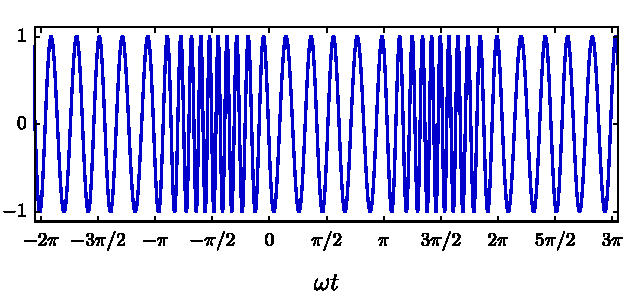
\includegraphics[scale=1]{2-ARM-theory/Figures/figure2A.pdf}
  \caption[Oscillatory factors of the SFA integrand prior to the saddle-point approximation]{%
  Real part of the oscillatory factors of Eq.~\eqref{e2-yield-after-order-switch}, for a sinusoidal field of the form $A(t)=-\frac{F}{\omega}\sin(\omega t)$.
  Here the field strength is $F=\SI{\figuretwoAfield}{\au}$, for a $\lambda= \SI{\figuretwoAlambda}{nm}$ field ionizing \figuretwoAtarget{} into a final momentum of $p=\SI{\figuretwoAmomentum}{\au}$
  }
  \label{f2-oscillatory-factors}
\end{figure}
%%% Note hackish a.u. - period interaction at the end there.


The solution is to use what is known as the \textit{saddle-point approximation}. If the integrand is an analytic function of $t'$, we can deform the path of integration to any path that connects the two endpoints and obtain the same integral, so we can look for better choices of integration contour. The basic features of the integrand are captured mainly by the oscillatory factors, $e^{i I_{p,n} t'} e^{\frac{i}{2} \int_T^{t'} \left(\vbp+ \vba(\tau) \right)^2\d\tau}=e^{-iS(t')}$, whose structure is shown in \reffig{f2-saddle-points-3d}. 

\begin{figure}[t!]
  \centering
  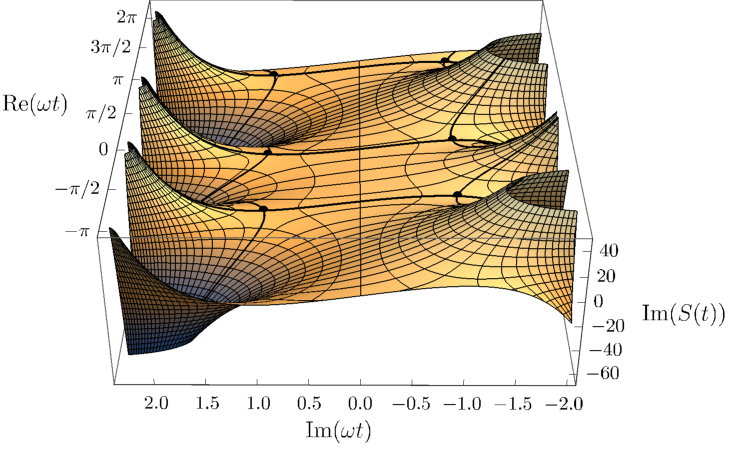
\includegraphics[scale=1]{2-ARM-theory/Figures/figure2B.pdf}
  \caption[Landscape of the imaginary action $\Im(S(t))$ over imaginary time, showing the steepest-descent contours]{%
    Landscape for the amplitude of the exponent in the oscillatory factors, $e^{-iS(t')}=e^{i I_p t'} e^{\frac{i}{2} \int_T^{t'} \left(p+ A(\tau) \right)^2\d\tau}$, for the same field as \reffig{f2-oscillatory-factors}. The height and colour of the landscape indicate $\Im(S(t'))$, which governs the amplitude of the integrand through $|e^{-iS(t')}|=e^{\Im{S(t')}}$. The lines of constant $\Re(S(t'))$ are orthogonal to the $\Im(S(t'))$ contour lines, and they form the paths of steepest ascent and descent on the landscape, along which $e^{-iS(t')}$ ceases to oscillate, changing only in amplitude.
  }
  \label{f2-saddle-points-3d}
\end{figure}


In particular, if we shift the contour towards positive imaginary times, the amplitude of the oscillations, given by $|e^{-iS(t')}|=e^{\Im\left(S(t')\right)}$ decreases sharply except for a few points of maximal contribution, and if we make the contour pass through the saddle points of the landscape (the solutions of the complex equation $\frac{\d S(t')}{\d t'}=0$), we minimize the maximal amplitude of the integrals. In addition to this, we can also choose an integration contour along the lines where the $\Re(S(t'))$ is constant, which guarantees that the amplitude drop is as fast as possible and that the oscillations stop; the integrand $e^{-iS(t')}$ then becomes a series of sharp, flat, gaussian-like humps centred on each of the saddles. 

So far, this procedure can be done exactly, and it provides a way to neutralize the effect of the integrand's oscillations at the cost of finding a complicated contour and integrating over it. The saddle-point approximation itself consists of forgetting about the long tails of the contour in the valleys of the integrand, and seeing the transformed integrand for what it is: a series of humps which are very well approximated by gaussians that can be integrated exactly, leaving a single contribution from each hump.


\pagebreak
\begin{mathaside}{The saddle-point approximation}
\label{aside.SPA}
\noindent
More precisely, if $F$ is an analytic function which varies slowly with respect to the analytic exponent $\varphi$, then the integral of the combination $e^{\rho \varphi(\zeta)}$ can be approximated by a sum of the form
\begin{equation}
\int_A^B F(\zeta) e^{\rho \varphi(\zeta)}\d\zeta
=
\sum_s
\sqrt{\frac{2\pi}{\rho}} 
\frac{F(\zeta_s) e^{\rho\varphi(\zeta_s)}}{\left[-\varphi''(\zeta_s)\right]^{1/2}}
\label{e2-SPA-statement}
\end{equation}
over all the relevant saddle points $\zeta_s$, which satisfy $\varphi'(\zeta_s)=0$ and are accessible to a deformed contour that joins $A$ and $B$~\cite{BruijnAsymptotics, Bleistein_Integrals, GerlachSPAonline}. In general this approximation holds in an asymptotic sense as the multiplier increases to $\rho\to\infty$, which is missing from our exponent, but in practice the exponent is large enough that the saddle-point approximation is excellent.
\end{mathaside}




Turning back to our integral, we see that the temporal integral 
\begin{align}
\int_{-\infty}^{\tn}\!\d t'
e^{-i\left(\vbp+\vba(t')\right)\cdot\vb{r}
 +i I_{p,n} t'
 +\frac{i}{2} \int_T^{t'}\left(\vbp+\vba(\tau)\right)^2\d\tau}
e^{i\int_T^{t'} U_n(\rl(\tau;\vb{r},\vbp,t'))\d\tau}
\label{e2-temporal-integral-before-saddle-point}
\end{align}
naturally splits into two components: a slow-acting Coulomb phase $e^{i\int_T^{t'} U_n(\rl(\tau;\vb{r},\vbp,t'))\d\tau}$ and a fast oscillatory factor $e^{-iS_V(t')}$ where the phase is given by the classical action of an electron in the field, 
\begin{equation}
S_V(t')
=
\left(\vbp+\vba(t')\right)\cdot\vb{r}
-I_{p,n} t'
-\frac{1}{2} \int_T^{t'}\left(\vbp+\vba(\tau)\right)^2\d\tau,
\label{e2-volkov-action-definition}
\end{equation}
which we will generally call the Volkov action.

The saddle-point approximation then asks us to look for the points at which this phase is stationary, which happens when
\begin{align}
0 & =
\frac{\d S_V}{\d t'}(\tvr)
=
\frac{\d}{\d t'}\left[-\frac{1}{2} \int_T^{t'}\left(\vbp+\vba(\tau)\right)^2\d\tau- I_{p,n} t'+\left(\vbp+\vba(t')\right)\cdot\vb{r}\right]_{\tvr}
\nonumber \\ & = 
-\left(\frac{1}{2} \left(\vbp+\vba(\tvr)\right)^2+ I_{p,n} + \vbf(\tvr)\cdot\vbr\right)
.
\end{align}
This condition is relatively complicated, because the equation, and therefore also the solution,~$\tvr$, depends on the position $\vbr$, which will later be integrated over. To tackle this, we will concentrate on a `central' saddle point, which satisfies the equation
\begin{equation}
\frac{1}{2} \left(\vbp+\vba(\ts)\right)^2+ I_{p,n}=0,
\label{e2-ts-equation}
\end{equation}
and then we will estimate the effect of the additional terms $\vbf(\tvr)\cdot\vbr$ on~$\tvr$. In general, if the boundary radius is chosen well inside the tunnelling region, which occurs when
\begin{equation}
|Fa|\ll I_{p,n},
\label{e2-Fa-Ip-restriction}
\end{equation}
then $\tvr$ will be close to $\ts$ and we will be able to estimate the effect of the term $\vbf(\tvr)\cdot\vbr$ in a linearized regime.


For the monochromatic, linearly polarized fields we consider, the saddle-point equation \eqref{e2-ts-equation} is easy to solve. Separating the momentum into its parallel and orthogonal components with respect to the laser polarization, and taking 
\begin{equation}
\vba(t)=-\frac{F}{\omega}\un \sin(\omega t),
\label{e2-field-definition}
\end{equation}
the saddle-point equation reads
\begin{equation}
\frac{1}{2} \left(\pp -\frac{F}{\omega}\sin(\omega \ts) \right)^2 +\frac{1}{2}\pt^2 + \frac 12 \kappa_n^2=0,
\end{equation}
for $\kappa_n=\sqrt{2I_{p,n}}$, or, alternatively,
\begin{equation}
\pp -\frac{F}{\omega}\sin(\omega \ts)
=\pm\sqrt{-(\kappa_n^2+\pt^2)},
\end{equation}
which is easily resolved to 
\begin{equation}
\omega \ts
= \arcsin\left(
\frac{\omega}{F}\left(\pp\pm i \sqrt{\kappa_n^2+\pt^2}\right)
\right).
\end{equation}
Here the arcsine function is a standard holomorphic function \citenistsec{4.23}, whose principal branch has branch cuts on $(-\infty,-1]$ and $[1,\infty)$, and takes values in the complex strip $-\frac{\pi}{2}<\Re(\arcsin(\zeta))<\frac{\pi}{2}$. In particular, the arcsine function takes the upper half-plane $\Im(\zeta)>0$ into the upper half-strip $\Im(\arcsin(\zeta))>0$, and since we're only interested in saddle-point times $\ts$ with positive imaginary parts -- as those are the ones that give acceptable contours, as shown in \reffig{f2-oscillatory-factors} -- we can finally take only the positive sign to~get
\begin{equation}
\omega \ts
= \arcsin\left(
\frac{\omega}{F}\left(\pp + i \sqrt{\kappa_n^2+\pt^2}\right)
\right).
\label{e2-saddle-point-equation-final-solution}
\end{equation}


To solve the full equation for $\tvr=\ts+\Delta \tvr$, we linearize the equation at $\ts$, which reads
\begin{equation}
\vba(\tvr)
=\vba(\ts +\Delta\tvr)
\approx \vba(\ts) + \Delta\tvr\frac{\d\vba}{\d t}(\ts)
=\vba(\ts) - \Delta\tvr \vbf(\ts)
\end{equation}
and a similar expansion for $\vbf(\tvr)$, to get 
\begin{align}
0
& = 
\frac{1}{2} \left(\vbp+\vba(\ts)-\Delta t_a\vbf(\ts)\right)^2+ I_{p,n} + \vbf(\ts)\cdot\vbr +\Delta t_a\frac{\d\vbf}{\d t}(\ts)\cdot\vbr 
\nonumber \\ & = 
\frac{1}{2} \left(\vbp+\vba(\ts)\right)^2+ I_{p,n}  -\Delta t_a\left(\vbp+\vba (\ts) \right) \cdot\vbf(\ts) + \vbf(\ts)\cdot\vbr 
\nonumber \\   & \qquad+
\frac{1}{2} \left(\Delta t_a\vbf(\ts)\right)^2  +\Delta t_a\frac{\d\vbf}{\d t}(\ts)\cdot\vbr
\nonumber \\ & = 
\Delta t_a\left(\frac{\d\vbf}{\d t}(\ts)\cdot\vbr-\left(\vbp+\vba(\ts)\right)\cdot\vbf(\ts) \right) + \vbf(\ts)\cdot\vbr 
%\nonumber \\   & \qquad+
+\frac{1}{2} \left(\Delta t_a\vbf(\ts)\right)^2 
.
\end{align}
Dropping the quadratic term for consistency, we get $\Delta\tvr$ in the form
\begin{equation}
\Delta\tvr
= \frac{\vbr\cdot\vbf(\ts)}{\left(\vbp+\vb{A}(\ts)\right)\cdot\vbf(\ts)}
=\frac{z}{\pp+A(\ts)},
\end{equation}
where $z=\vbr\cdot\un$ is the position coordinate along the laser polarization. Here, we should note that the denominator in this expression, $\pp+A(\ts)$, gives the kinematic momentum -- equal to the velocity $\vp(\ts)$, since the mass is unity -- at the time of ionization $\ts$. Moreover, this kinematic momentum is completely determined by the saddle-point equation \eqref{e2-saddle-point-equation-final-solution},~as 
\begin{equation}
\vp(\ts)=\pp+A(\ts)=-i\sqrt{ \kappa_n^2+\pt^2} \approx -i\kappa_n.
\label{e2-vp-as-i-kappa}
\end{equation}
Finally, the position $z=\vbr\cdot\un$ in the numerator is bounded, since the $\vbr$ integral is to be taken only over the ARM boundary of radius $a$.


We can now begin using these tools to simplify our integral, which with the application of the saddle-point approximation reads
\begin{align}
& a_n^{(0)}(\vb{p},\tn)
 =
-i e^{-iE_n\tn} 
\int\frac{\d\vbr}{(2\pi)^{3/2}}
\matrixel{\vbr}{\hat{L}^{(-)}(a)}{n_D}
\int_{-\infty}^{\tn}\!\d t'
e^{-iS_V(t')}
e^{i\int_T^{t'} U_n(\rl(\tau;\vb{r},\vbp,t'))\d\tau}
\nonumber \\ & \qquad \approx 
-i e^{-iE_n\tn} 
\int\frac{\d\vbr}{(2\pi)^{3/2}}
\matrixel{\vbr}{\hat{L}^{(-)}(a)}{n_D}
\sqrt{\frac{2\pi}{iS_V''(\tvr)}}
e^{-iS_V(\tvr)}
e^{i\int_T^{\tvr} U_n(\rl(\tau;\vb{r},\vbp,\tvr))\d\tau}
.
\label{e2-yield-after-saddle-point-approximation}
\end{align}
Here it is important to note that we are focusing on the contribution from a \textit{single} burst of ionization, represented by the selection of the contribution of a single saddle point. To get the full contribution, one must select all relevant saddle points and add their contributions coherently, which then gives rise to both inter-cycle interference -- otherwise known as ATI rings -- and intra-cycle interferences which provide additional structure to the photoelectron spectrum. In this thesis, however, we will focus on the details of the contribution of each specific ionization burst.


For now, we focus on analysing the contribution of the phase $e^{-iS_V(\tvr)}$, which we can again linearize with respect to the saddle point displacement $\Delta\tvr$ to get
\begin{align}
S_V(\tvr) & =S_V(\ts) + \Delta\tvr S_V'(\ts)
\\ \text{with}\quad
S_V'(\ts) & =
\frac{\d\vba}{\d t}(\ts)\cdot\vbr
-I_{p,n}
-\frac{1}{2} \left(\vbp+\vba(\ts)\right)^2
=
-\vbf(\ts)\cdot\vbr,
\end{align}
and with 
\begin{equation}
S_V(\ts)
=
\left(\vbp+\vba(\ts)\right)\cdot\vb{r}
-I_{p,n} \ts
-\frac{1}{2} \int_T^{\ts}\left(\vbp+\vba(\tau)\right)^2\d\tau
\end{equation}
separating into an $\vbr$-dependent component, $\left(\vbp+\vba(\ts)\right) \cdot \vbr$, and an $\vbr$-independent one, $I_{p,n} \ts + \frac{1}{2} \int_T^{\ts} \left(\vbp+\vba(\tau) \right)^2 \d\tau$. On the other hand, since it appears in a pre-exponential factor, we neglect the appearance of $\tvr$ in the square root and take $S_V''(\tvr) \approx S_V''(\ts)$.

Putting these in place, then, we can now separate the main position-independent parts from the position integral, which reads
\begin{align}
a_n^{(0)}(\vb{p},\tn)
& =
\frac{-i e^{-iE_n\tn}}{\sqrt{iS_V''(\ts)}}
e^{iI_{p,n} \ts + \frac{i}{2} \int_T^{\ts}\left(\vbp+\vba(\tau)\right)^2\d\tau }
\nonumber \\ & \quad \times
\int\frac{\d\vbr}{2\pi}
e^{-i \Delta\tvr S_V'(\ts)}
e^{i\int_T^{\tvr} U_n(\rl(\tau;\vb{r},\vbp,\tvr))\d\tau}
e^{-i\left(\vbp+\vba(\ts)\right)\cdot\vb{r}}
\matrixel{\vbr}{\hat{L}^{(-)}(a)}{n_D}
.
\label{e2-yield-after-rearrangement}
\end{align}
Here, moreover, we neglect the term  in $\Delta\tvr S_V'(\ts)$, which is of order $Fa^2/\kappa_n$, as it is second-order in $a$. This represents the strongest upper bound on our boundary radius, which is then restricted by
\begin{equation}
\kappa_n a \gg 1
\qq{and}
Fa^2\ll \kappa_n.
\end{equation}
The two together then imply that $Fa \ll \kappa_n/a \sim I_{p,n}/\kappa a \ll I_{p,n}$. They also imply a restriction on the strength of the field the theory is able to handle, as $F \ll \kappa_n/a^2 \ll \kappa_n^3$, which is the characteristic electric field strength for the state $\ket{n}$.


To go further, we now need to look directly at the Bloch matrix element with the Dyson orbital, $\matrixel{\vbr}{\hat{L}^{(-)}(a)}{n_D}$. Substituting in the definition~\eqref{e2-bloch-operator-with-function} gives us 
\begin{equation}
\matrixel{\vbr}{\hat{L}^{(-)}(a)}{n_D}
=
\delta(r-a)\left( \frac{\partial}{\partial r} + b(r) \right)
\braket{\vbr}{n_D},
\end{equation}
but to go beyond that we need some kind of additional handle on the Dyson orbital and its radial dependence. To get such a handle, we use the fact that we are taking the ARM artificial boundary to be far from the core, so $\kappa_n a \gg 1$, and in this regime the wavefunction is in its asymptotic regime, where only a single electron is likely to be present at any given time, and its wavefunction is in the semiclassical WKB regime, of the form
\begin{equation}
\psi_g(r=a) \propto e^{-i\int_{\tvr}^{\tk}U\d\tau}.
\label{e2-ground-state-WKB-dependence}
\end{equation}



General results regarding this connection are hard to establish analytically, although numerical methods based on ensembles of wavepackets propagated classically are quite successful \cite{Tannor_time_dependent_QM}. This is due partly to the difficulty of constructing WKB methods%
\footnote{Wentzel–Kramers–Brillouin methods; see e.g. \citer{cohen-tannoudji_QM}.}
on more than one spatial dimension, and also to the fact that the Dyson orbital $\ket{n_D(t)}=\sqrt{N}\braket{n(t)}{\Psi_g}$ depends on far more detail on the neutral and ionic hamiltonians than through the mean value $U_n=\matrixel{n(t)}{V_{ee}}{n(t)}$. 

The general plan is to match this WKB expression to the $\tvr$-dependent Coulomb phase $e^{i\int_T^{\tvr} U_n(\rl(\tau;\vb{r},\vbp,\tvr))\d\tau}$ in the ionization yield integral, in the hope that the (unphysical) dependence on the boundary radius $a$ will vanish. In general this will be possible, but only approximately so, and it will be achieved by transforming both expressions to a common reference point.

Thus, we begin with the laser-driven trajectory from the argument of the electrostatic interaction $U_n$, which reads (using $\vbv(t)=\vbp+\vba(t)$ for simplicity)
\begin{align}
\rl(\tau;\vb{r},\vbp,\tvr)
& =
\vb{r}+\int_\tvr^\tau \vbv(\tau')\d\tau'
=
\vb{r}-\int^\tvr_{\ts} \vbv(\tau')\d\tau'+\int_{\ts}^\tau \vbv(\tau')\d\tau'
\nonumber \\ & \approx
\Big( \vb{r} - \Delta\tvr\vbv(\ts) \Big) + \int_{\ts}^\tau \vbv(\tau')\d\tau'.
\end{align}
In this form, it is easier to see that most of the directional contribution in the first two terms vanishes, because $\Delta\tvr = z/\vp(\ts)$ is essentially the time it takes for the electron to advance along the $z$ axis to the specified starting position at the birth velocity $\vp(\ts)$, even though both the time and the velocity are complex quantities. To make this argument more precise, we simply calculate the terms in brackets to get
\begin{align}
\vbr - \Delta\tvr \vb{v}(\ts)
= 
\vbr - \frac{\vbf(\ts)\cdot\vbr}{\vbf(\ts)\cdot\vbv(\ts)} \vbv(\ts) 
=
\begin{pmatrix}x\\y\\z\end{pmatrix} - \frac{z}{v_z}\begin{pmatrix}v_x\\v_y\\v_z \end{pmatrix}=\frac{1}{v_z}\begin{pmatrix}v_z x-v_x z\\v_z y-v_y z\\0\end{pmatrix},
\end{align}
where the first two components are strongly reminiscent of a vector cross product. Thus, as long as the main contributions to the spherical integral come from points that satisfy
\begin{equation}
\frac{x}{z}\approx \frac{v_x}{v_z}\textrm{ and }\frac{y}{z}\approx \frac{v_y}{v_z},
\end{equation}
we can ignore the remnant $\vbr - \Delta\tvr \vbv(\ts)$, which makes the inner integral $\vbr$-independent. It is important to note here, though, that $\vp(\ts) = \pp + A(\ts)$ is a complex quantity, whereas the transverse components are simply the transverse momentum and are therefore real, as are in this setting all three position coordinates. Nevertheless, this approximation is good enough that we will ignore the remnant. With this, then, we can approximate the inner integral in $U_n(\rl(\tau;\vb{r},\vbp,\tvr))$ as
\begin{equation}
e^{i\int_T^\tvr U_n(\rl(\tau;\vb{r},\vbp,\tvr))\d\tau}
\approx 
\exp\left[{-i\int_\tvr^T U_n\left(\int_{ \ts}^\tau \vb{v}(\tau')\d\tau'\right) \d\tau}\right].
\end{equation}


Finally, we split the outer integral up into two contributions, one from the $\vbr$-dependent $\tvr$ to some reference time $\tk$ that depends only on the initial state (which encapsulates the $\vbr$ dependence), and one from $\tk$ to the final time $T$ (which catches the bulk of the tunnelling dynamics), so 
\begin{equation}
e^{i\int_T^\tvr U_n(\rl(\tau;\vb{r},\vbp,\tvr))\d\tau}
\approx 
e^{-i\int_\tvr^\tk U_n\left(\int_{ \ts}^\tau \vb{v}(\tau')\d\tau'\right) \d\tau}
e^{-i\int_\tk^T U_n\left(\int_{ \ts}^\tau \vb{v}(\tau')\d\tau'\right) \d\tau}.
\end{equation}
This concludes the transformations of this factor, which when put back into our ionization yield~\eqref{e2-yield-after-rearrangement} gives 
\begin{align}
a_n^{(0)}(\vb{p},\tn)
& =
\frac{-i e^{-iE_n\tn}}{\sqrt{iS_V''(\ts)}}
e^{iI_{p,n} \ts + \frac{i}{2} \int_T^{\ts}\left(\vbp+\vba(\tau)\right)^2\d\tau }
e^{-i\int_\tk^T U_n\left(\int_{ \ts}^\tau \vb{v}(\tau')\d\tau'\right) \d\tau}
\nonumber \\ & \quad \times
\int\frac{\d\vbr}{2\pi}
e^{-i\int_\tvr^\tk U_n\left(\int_{ \ts}^\tau \vb{v}(\tau')\d\tau'\right) \d\tau}
e^{-i\left(\vbp+\vba(\ts)\right)\cdot\vb{r}}
\matrixel{\vbr}{\hat{L}^{(-)}(a)}{n_D}
.
\label{e2-ionization-yield-separated}
\end{align}


In one sense, we're done: this expression completes the separation of the temporal integral and the encapsulation of the shape-dependent factors. Indeed, we can now define
\begin{equation}
R_n(\vbp)
=
\frac{-i }{\sqrt{iS_V''(\ts)}}
\int\frac{\d\vbr}{2\pi}
e^{-i\int_\tvr^\tk U_n\left(\int_{ \ts}^\tau \vb{v}(\tau')\d\tau'\right) \d\tau}
e^{-i\left(\vbp+\vba(\ts)\right)\cdot\vb{r}}
\matrixel{\vbr}{\hat{L}^{(-)}(a)}{n_D},
\label{e2-shape-factor-definition}
\end{equation}
and this represents a shape factor that carries all the information about the shape of the molecular wavefunction, with only a relatively weak dependence on the tunnelling time $\ts$, giving an ionization yield of the form
\begin{align}
a_n^{(0)}(\vb{p},\tn)
& =
e^{-iE_n\tn}
e^{iI_{p,n} \ts + \frac{i}{2} \int_T^{\ts}\left(\vbp+\vba(\tau)\right)^2\d\tau }
e^{-i\int_\tk^T U_n\left(\int_{ \ts}^\tau \vb{v}(\tau')\d\tau'\right) \d\tau}
R_n(\vbp)
.
\label{e2-ionization-yield-with-shape-factor}
\end{align}
This contains the essential results of the Analytical $R$-Matrix theory of tunnelling in an explicit and simple fashion. Of course, more work is required on the shape factor -- essentially a Fourier transform of the Dyson orbital over the spherical boundary --, in terms of showing its independence with respect to the choice of the boundary radius $a$, but in practice this requires a more concrete Dyson orbital to really work. Nevertheless, in general, the Coulomb phase $e^{-i\int_\tvr^\tk U_n\left(\int_{ \ts}^\tau \vb{v}(\tau')\d\tau'\right) \d\tau}$ in $R_n(\vbp)$ will typically cancel out the radial $a$ dependence of the amplitude in $\matrixel{\vbr}{\hat{L}^{(-)}(a)}{n_D}$.



For completeness, we include here a brief analysis of the Volkov action's second derivative, $S_V''$. We know already the first derivative, 
\begin{align}
-i\frac{\d S_V}{\d t'}
 & = i\left(\frac{1}{2} \left(\vbp+\vba(t')\right)^2+ I_{p,n} + \vbf(t')\cdot\vbr\right),
\end{align}
from which we can calculate
\begin{align}
\frac{\d^2 S_V}{\d t'^2}
& = 
-\left(\left(\vbp+\vba(t')\right)\cdot\frac{\d\vba}{\d t'} + \frac{\d\vbf(t')}{\d t'}\cdot\vbr\right)
= 
\left(\vbv(t')\cdot\vb{F}(t') - \frac{\d\vbf(t')}{\d t'}\cdot\vbr\right).
\end{align}
The second term does depend on $\vbr$ but it is precisely this dependence that makes it negligible with respect to the first, as long as the product $a^2\omega$ is of order unity, for $\omega$ the pulse's carrier frequency. Under this approximation, then, $S_V''(\ts)$ depends only on the parallel momentum $p_\parallel$, and is equal in a semiclassical interpretation to the power delivered by the laser pulse to the ionized electron.





\subsection{The shape factor and boundary independence}
We now turn to examine the shape factor $R_n(\vbp)$ in more detail. As mentioned above, the definition~\eqref{e2-shape-factor-definition} does a good job of boxing up the dependence on the shape of the ionized Dyson orbital, but it is a complicated quantity and, more specifically, it has an explicit dependence on the choice of boundary radius $a$, which is arbitrary and should not affect any physical results. In general, the dependence from the wavefunction will cancel out with that from the eikonal Coulomb phase $e^{-i\int_\tvr^\tk U_n\left(\int_{ \ts}^\tau \vb{v}(\tau')\d\tau'\right) \d\tau}$, and in this section we will examine this claim for the specific example of an orbital for which the radial and angular dependence factor out.

More specifically, we consider the separable orbital
\begin{align}
\braket{\vbr}{n_D}
= 
\varphi(r) f(\theta,\phi)
\end{align}
where $f$ is arbitrary for now, and where the radial wavefunction $\varphi$ is in the asymptotic WKB regime for a state of ionization potential $I_{p}=\frac12 \kappa^2$ (dropping, for now, the subscript $n$) and charge $Q$,
\begin{equation}
\varphi(r) 
= 
C_{\kappa l} \kappa^{3/2} \frac{e^{-\kappa r}}{\kappa r}(\kappa r)^{Q/\kappa}.
\label{e2-radial-WKB-wavefunction}
\end{equation}



The first step is to deal with the action of the Bloch operator, where we can ignore the angular part of the wavefunction. Taking the definition \eqref{e2-bloch-operator-with-function}, we get the relatively simple expression
\begin{align}
\left.\left(\frac{\partial}{\partial r}+b(r)\right)\right|_{a} \varphi(r)
& = 
C_{\kappa l} \kappa^{3/2}\left.\left(\frac{\partial}{\partial r}+b(r)\right)\right|_{a} \left[ \frac{e^{-\kappa r}}{\kappa r}(\kappa r)^{Q/\kappa}\right]
\nonumber \\ & = 
C_{\kappa l} \kappa^{3/2}\left.\left(-\kappa-\frac{1}{a}+\frac{Q/\kappa}{a}+b(a)\right)\right. \left[ \frac{e^{-\kappa a}}{\kappa a}(\kappa a)^{Q/\kappa}\right]
\nonumber \\ & = 
\left(-\kappa+\frac{Q/\kappa-1}{a}+b(a)\right)\varphi(a).
\end{align}
Note that here we use the freedom in the choice of $b(r)$ to set it to
\begin{equation}
b(r) = \frac{1-Q/\kappa}{r},
\end{equation}
using $\kappa=\sqrt{2I_p}$ for the ionization potential to the ionic ground state, which guarantees that 
\begin{equation}
\matrixel{\vbr}{\hat{L}^{(-)}(a)}{n_D} = -\kappa \braket{\vbr}{n_D},
\label{e2-wkb-explicit-expression}
\end{equation}
for the ground state, with small corrections on that for higher-lying ionic states. The action of the Bloch operator then reduces to a constant, and we can focus on the wavefunction as per~\eqref{e2-radial-WKB-wavefunction}.

This WKB expression is to be matched by the eikonal Coulomb phase, which corresponds in this case to a bare Coulomb interaction with a charge $Q$,
\begin{equation}
U_n(\vbr)\approx -\frac{Q}{r}.
\end{equation}
As such, its integral is given by 
\begin{align}
-i\int_{\tvr}^{\tk}U_n\left(\int_{ \ts}^\tau \vb{v}(\tau')\d\tau',\tau\right) \d\tau = \int_{t_a}^{\tk} \frac{-iQ\d\tau}{\sqrt{r(\tau)^2}}
\label{e2-WKB-integral-coulomb}
\end{align}
where we have defined $r(\tau)\colonequals \int_{ \ts}^\tau \hat{\vbr}\cdot\vb{v}(\tau')\d\tau'$, for which $\frac{\d r}{\d\tau}=\hat{\vbr}\cdot \vb{v}(\tau).$ To proceed, we now perform two approximations: we first assume that the velocity will not change significantly during the time interval being integrated, so we can replace $\vb{v}(\tau)$ by $\vb{v}(\ts)$, and we further suppose that the tunnelling velocity will be primarily directed towards negative $z$ (since the field points towards positive $z$ and the charge is negative). These two together imply that $\frac{\d r}{\d\tau}\approx-v_\parallel(\ts)\approx+i\kappa$ and therefore that
\begin{align}
\int_{\tvr}^{\tk} \frac{-iQ\d\tau}{\sqrt{r(\tau)^2}}
=
-\frac{Q}{\kappa}\int_{a}^{r_\kappa} \frac{\d r}{\sqrt{r^2}}
=
+\frac{Q}{\kappa}\int_{a}^{r_\kappa} \frac{\d r}{r}
=
\frac{Q}{\kappa}\ln\left(\frac{r_\kappa}{a}\right)
=
-\frac{Q}{\kappa}\ln\left(\kappa a\right),
\end{align}
where the radial constant $r_\kappa$, equal to the radius at the originally arbitrary integration limit $\tk$, has been chosen as $r_\kappa=1/\kappa$. The exponential of this integral, 
\begin{equation}
e^{
-i\int_{\tvr}^{\tk}U_n\left(\int_{ \ts}^\tau \vb{v}(\tau')\d\tau'\right) \d\tau 
}
=
e^{
-\frac{Q}{\kappa}\ln\left(\kappa a\right)
}
=(\kappa a)^{-Q/\kappa},
\end{equation}
is then a direct counterpart to the equivalent factor in~\eqref{e2-radial-WKB-wavefunction}.

We can thus incorporate all of this into the shape factor~\eqref{e2-shape-factor-definition}, to get 
\begin{equation}
R_n(\vbp)
=
\frac{ iC_{\kappa l} \kappa^{5/2} }{\sqrt{iS_V''(\ts)}}
\frac{e^{-\kappa a}}{\kappa a}
\int\frac{a^2\d\Omega}{2\pi}
f(\theta,\phi)
\left. e^{-i\left(\vbp+\vba(\ts)\right)\cdot\vb{r}} \right|_{r=a}
. 
\label{e2-shape-factor-first-stab}
\end{equation}
This is a Fourier transform of the angular dependence taken over the spherical boundary, but it is important to note that the momentum of the Fourier transform, $\vbp+\vba(\ts)$, is in general a complex vector since the ionization time $\ts$ is also complex; this will change the phase to an exponential which will counter the existing $e^{-\kappa a}$ from the wavefunction.

In fact, because the complex ionization time $\ts$ is a tightly-controlled function of the momentum, via the saddle-point equation \eqref{e2-ts-equation}, the exponential factor $\vbp+\vba(\ts)$ has very little freedom, and it does not actually depend on the longitudinal momentum $\pp$ along the laser polarization. Splitting that vector in its components along and across the laser polarization,
\begin{equation}
\vbp+\vba(\ts) = \vbpo + (\pp + A(\ts))\un,
\end{equation}
with $\vbpo\cdot\un=0$, the saddle-point equation~\eqref{e2-ts-equation} reads
\begin{equation}
\frac 12 \pt^2 + \frac12 (\pp + A(\ts))^2 = - \frac12 \kappa^2.
\end{equation}
Here we must choose the imaginary sign for the square root, because those are the roots that can be reached with the appropriate contours shown in \reffig{f2-saddle-points-3d}
with the negative imaginary sign chosen for the square root, so that 
\begin{equation}
\pp + A(\ts) = -i \sqrt{\kappa^2 + \pt^2},
\end{equation}
and therefore
\begin{equation}
\vbp+\vba(\ts) = \vbpo -i \sqrt{\kappa^2 + \pt^2} \un.
\end{equation}
With this, then, the shape factor simplifies to
\begin{equation}
R_n(\vbp)
=
\frac{ iC_{\kappa l} \kappa^{1/2} }{\sqrt{iS_V''(\ts)}}
\kappa a \, e^{-\kappa a}
\int\frac{\d\Omega}{2\pi}
f(\theta,\phi)
e^{-i a\vbpo \cdot\ur } 
e^{-\kappa a\sqrt{1 + \pt^2/\kappa^2} \un \cdot\ur } 
,
\label{e2-shape-factor-second-stab}
\end{equation}
for $\ur=\vbr/r$ the unit vector along $\vbr$. Here the last factor $e^{-\kappa a\sqrt{1 + \pt^2/\kappa^2} \un \cdot\ur } \approx e^{-\kappa a \un \cdot\ur }$ concentrates the integral along positions opposite to the laser polarization direction $\un$, that is, positions where $\un\cdot\ur \approx -1$, and where therefore that factor is of the order of $e^{\kappa a}$. This will then cancel out with the $e^{-\kappa a}$ factor from the wavefunction.

Finally, there is an additional factor of $a$ that comes from the geometrical factors of the wavefunction and the volume element, and this too will in general cancel out. Here, though, the internal dependence is via the scale embedded in the Fourier kernel $e^{-i a\vbpo \cdot\ur }$, so the effect must be seen on a case-by-case basis. Nevertheless, we expect from the $a$ independence of $R_n(\vbp)$ that the integral will have a leading dependence on $a$ of the form~$e^{\kappa a}/\kappa a$.

To wrap up this section, we encapsulate this inner integral in its own notation, as 
\begin{subequations}
\begin{align}
R_n(\vbp)
 =
\frac{ iC_{\kappa l} \kappa^{3/2} }{\sqrt{iS_V''(\ts)}}
a
e^{-\kappa a}
\sft(\vbq),  &
\label{e2-shape-factor-via-sft}
\\ \text{where} \ 
\sft(\vbq)
& =
\int\frac{\d\Omega}{2\pi}
f(\theta,\phi)
e^{-i \vbq\cdot\ur } 
\label{e2-sft-definition}
,
\end{align}
\end{subequations}
for $\vbq=a(\vbp+\vba(\ts))=a\vbpo -i \kappa a \sqrt{1+\pt^2/\kappa^2}\:\un$. To be able to say more about this spherical Fourier transform, though, we require a better handle on the ingredients -- we need an explicit angular wavefunction.







\section{Molecular shape factors}
\label{sec:molecular-shape-factors}
One useful test case for this Fourier transform is the case of hydrogenic orbitals, which are easy to treat analytically and which afford fairly clean (but still approximate) results that can be matched against the existing PPT theory~\cite{perelomov_ionization-III_1967}, which is the approach taken in Refs.~\citealp{ MResReport} and~\citealp{ARM_initial}. As an alternative to that, here we will treat a more complex molecular shape, and we will focus on an angular dependence of the form
\begin{subequations}
\begin{align}
f(\theta,\phi) & = F(\cos(\theta), \sin(\theta)\cos(\phi))
, \quad \text{for}\\ 
F(\cos(\theta), \sin(\theta)\cos(\phi))
& = 
\cosh(b\cos(\theta)) (1+c\cos^2(\theta))  
\nonumber \\ & \qquad \times
\sin^{n_x+n_y}(\theta)\cos^{n_x}(\phi)\sin^{n_y}(\phi)  \cos^{n_z}(\theta)
.
\end{align}
\end{subequations}
This is a good model for the asymptotic angular dependence of molecular orbitals in small linear molecules \cite{radzig_reference_data, murray_tunnel_ionization_2011}, such as carbon dioxide or molecular nitrogen, and it describes an elongated orbital with one or no nodes in the molecular-frame $x$, $y$ and $z$ planes (according to whether $n_x$, $n_y$ and $n_z$ are $0$ or $1$, respectively), with the molecular axis along the $z$ direction. Here $\theta$ and $\phi$ are the azimuthal and longitudinal spherical coordinates in this molecular frame. In this section we will calculate the spherical Fourier transform of this orbital shape, obtaining simple analytical formulas for the shape factor of molecular orbitals.

Thus, we consider the integral
\begin{align}
\sft(\vbq)
=
\int\frac{\d\Omega}{2\pi}
&
\cosh(b\cos(\theta)) (1+c\cos^2(\theta))  
\sin^{n_x+n_y}(\theta)\cos^{n_x}(\phi)\sin^{n_y}(\phi)  \cos^{n_z}(\theta)
\nonumber \\ & \times 
e^{-i (q_x\sin(\theta)\cos(\phi) + q_y\sin(\theta)\sin(\phi) + q_z\cos(\theta) )}
,
\end{align}
which splits naturally into azimuthal and longitudinal integrals as
\begin{align}
\sft(\vbq)
=
&
\int_0^\pi\!\!\d\theta
\cosh(b\cos(\theta)) (1+c\cos^2(\theta))  
\sin^{n_x+n_y}(\theta)  \cos^{n_z}(\theta)
e^{-i q_z\cos(\theta) }
\nonumber \\ & \quad \times 
\frac{1}{2\pi}
\int_0^{2\pi}\!\!\d\phi
\cos^{n_x}(\phi)\sin^{n_y}(\phi)
e^{-i (q_x\sin(\theta)\cos(\phi) + q_y\sin(\theta)\sin(\phi) )}
.
\label{e2-sft-as-split-integrals}
\end{align}


Here the longitudinal integral is essentially a standard Bessel integral, but in practice this gets complicated by the mixed $\cos(\phi)$-$\sin(\phi)$ character of the exponent. To resolve this, we rewrite the momentum $\vbq$ in cylindrical coordinates, as
\begin{subequations}
\begin{empheq}[left=\empheqlbrace]{align}
q_x & = q_t \cos(\phi_q), \\
q_y & = q_t \sin(\phi_q).
\end{empheq}%
\label{e2-q-vector-in-cylindrical-coords}%
\end{subequations}%
It is important to note, however, that in general $\vbq$ will be a complex vector, and the characterization in~\eqref{e2-q-vector-in-cylindrical-coords} is only unambiguous for a real vector. The way to resolve this (which will be much-used tool throughout this section) is to assume that all quantities are real whenever they need to be, and then use analytic continuation to lift that restriction. This works because the integrand in~\eqref{e2-sft-as-split-integrals} is a continuous and entire function of the components of $\vbq$, integrated over a compact domain, so it has a unique analytical continuation to the whole of $\mathbb C^3$. If we can manipulate the integral, even if only for real parameters, into an explicitly analytical function of $q_x$, $q_y$ and $q_z$, the two forms must match over the extended complex domain.

The cylindrical decomposition in~\eqref{e2-q-vector-in-cylindrical-coords} helps us rephrase the exponential kernel of the longitudinal integral as $e^{-i (q_x\sin(\theta)\cos(\phi) + q_y\sin(\theta)\sin(\phi) )}=e^{-iq_t\sin(\theta)\cos(\phi-\phi_q)}$, but we still have to include the nodal factors in a standard way; this can be done via the identity
\begin{align}
\cos^{n_x}(\phi)\sin^{n_y}(\phi)
=
\left(\frac{e^{i\phi}+e^{-i\phi}}{2}\right)^{n_x}
\left(\frac{e^{i\phi}-e^{-i\phi}}{2i}\right)^{n_y}
\!\!=
\frac{
 e^{i(n_x+n_y)\phi} + (-1)^{n_x+n_y} e^{-i(n_x+n_y)\phi}
 }{
 2^{n_x+n_y}i^{n_y} + \delta_{n_x0}\delta_{n_y0}
 }
,
\end{align}
which is valid case-by-case for $0\leq n_x, n_y \leq 1$. Then, using Bessel's first integral~\citenisteq{10.9.2}, we have
{\allowdisplaybreaks
\begin{align}
\frac{1}{2\pi}
\int_0^{2\pi}\!\!\d\phi
&
\cos^{n_x}(\phi)\sin^{n_y}(\phi)
e^{-i (q_x\sin(\theta)\cos(\phi) + q_y\sin(\theta)\sin(\phi) )}
\nonumber \\ & =
\frac{1}{2\pi}
\int_0^{2\pi}
\frac{
 e^{i(n_x+n_y)\phi} + (-1)^{n_x+n_y} e^{-i(n_x+n_y)\phi}
 }{
 2^{n_x+n_y}i^{n_y} + \delta_{n_x0}\delta_{n_y0}
 }
e^{-iq_t\sin(\theta)\cos(\phi-\phi_q)}
\d\phi
\nonumber \\ & =
(-i)^{n_x+n_y}
\frac{
 e^{i(n_x+n_y)\phi_q} + (-1)^{n_x+n_y} e^{-i(n_x+n_y)\phi_q}
 }{
 2^{n_x+n_y}i^{n_y} + \delta_{n_x0}\delta_{n_y0}
 }
J_{n_x+n_y}(q_t\sin(\theta))
\nonumber \\ & =
(-i)^{n_x+n_y}
\cos^{n_x}(\phi_q)\sin^{n_y}(\phi_q)
J_{n_x+n_y}(q_t\sin(\theta))
\nonumber \\ & =
(-i)^{n_x+n_y}
\frac{ q_x^{n_x} q_y^{n_{\smash[b]{y}}}  }{(q_x^2+q_y^2)^\frac{n_x+n_y}{2}}
J_{n_x+n_y}\left(\sqrt{q_x^2+q_y^2}\sin(\theta)\right)
.
\label{e2-shape-factor-longitudinal-integral-to-bessel}
\end{align}
}%close \allowdisplaybreaks
As noted above, the equality holds for all real $q_x$ and $q_y$, with entire functions on both sides, so the two must match for all complex $q_x$ and $q_y$.

Using this expression, we can now phrase $\sft(\vbq)$ in the form
\begin{align}
\sft(\vbq)
=
&
\int_0^\pi\!\!\d\theta
\cosh(b\cos(\theta)) (1+c\cos^2(\theta))  
\sin^{n_x+n_y}(\theta)  \cos^{n_z}(\theta)
e^{-i q_z\cos(\theta) }
\nonumber \\ & \quad \times 
(-i)^{n_x+n_y}
\frac{ q_x^{n_x} q_y^{n_{\smash[b]{y}}}  }{(q_x^2+q_y^2)^\frac{n_x+n_y}{2}}
J_{n_x+n_y}\left(\sqrt{q_x^2+q_y^2}\sin(\theta)\right)
,
\label{e2-sft-with-longitudinal-bessels}
\end{align}
and begin the azimuthal integral. This integral is relatively complicated, but to make it somewhat simpler we can expand the hyperbolic cosine, $\cosh(b\cos(\theta))$, and include it into the Fourier kernel:
\begin{align}
\sft(\vbq)
=
&
\sum_\pm
\int_0^\pi\!\!\d\theta
(1+c\cos^2(\theta))  
\sin^{n_x+n_y}(\theta)  \cos^{n_z}(\theta)
e^{-i (q_z \pm i b)\cos(\theta) }
\nonumber \\ & \quad \times 
\frac{(-i)^{n_x+n_y}}{2}
\frac{ q_x^{n_x} q_y^{n_{\smash[b]{y}}}  }{(q_x^2+q_y^2)^\frac{n_x+n_y}{2}}
J_{n_x+n_y}\left(\sqrt{q_x^2+q_y^2}\sin(\theta)\right)
.
\label{e2-sft-with-cosh-substitution}
\end{align}


In this form, the integral is not that complicated, and it consists of the Fourier kernel $e^{-i (q_z \pm i b)\cos(\theta) }$, a Bessel function of the form $J_{n_x+n_y}\left(q_t \sin(\theta)\right)$, and a trigonometric polynomial in $\theta$. As such, the form is well covered by Gegenbauer's finite integral~[\citealp{watson_bessel_functions},~p.~379; \citealp{gradshteyn_ryzhik},~\S7.333], which reads
\begin{align}
\int_0^\pi
e^{iz\cos(\psi)\cos(\theta)}
&  
J_{\nu-\frac12}(z\sin(\psi)\sin(\theta))
C_r^{(\nu)}(\cos(\theta))
\sin^{\nu+\frac12}(\theta)
\:\d\theta
\nonumber \\ & \qquad \quad  =
\left(\frac{2\pi}{z}\right)^{1/2}
i^r
\sin^{\nu-\frac12}(\psi)
C_r^{(\nu)}(\cos(\psi))
J_{\nu+r}(z)
.
\label{e2-gegenbauer-integral}
\end{align}
Here the $C_r^{(\nu)}$ are Gegenbauer polynomials~\citenistsec{18.3} (also known as ultraspherical polynomials), and the formula is valid under $\Re(\nu)>-1$. The match is then easy to do, with $\nu=n_x+n_y+\frac12$, and setting
\begin{equation}
\left\{\begin{aligned}
z&=\sqrt{(q_z \mp ib)^2 +q_t^2}, \\
\psi&=\arctan\left(\frac{q_t}{\pm i b-q_z}\right),
\end{aligned}\right.
\longleftrightarrow
\left\{\begin{aligned}
\cos(\psi)&=\frac{\pm i b-q_z}{\sqrt{(q_z \mp ib)^2 +q_t^2}}, \\
\sin(\psi)&=\frac{q_t}{\sqrt{(q_z \mp ib)^2 +q_t^2}}.
\end{aligned}\right.
\end{equation}

The Gegenbauer polynomials themselves, though, need to be used as a basis for expressing the trigonometric polynomial $(1+c\cos^2(\theta)) \cos^{n_z}(\theta)$, and the form of  this depends on whether the polynomial is even or odd:
\begin{subequations}
\begin{equation}
\phantom{\cos(\theta)}
1+c\cos^2(\theta)
= 
\left(1+\frac{c}{2(\nu+1)}\right) 
C_0^{(\nu)}(\cos(\theta))
+
\frac{c}{2\nu(\nu+1)}
C_2^{(\nu)}(\cos(\theta))
\end{equation}
for $n_z=0$, and
\begin{equation}
\left[1+c\cos^2(\theta)\right] \cos(\theta)
= 
\left(\frac{1}{2\nu}+\frac{3c}{4\nu(\nu+2)}\right) 
C_1^{(\nu)}(\cos(\theta))
+
\frac{3c}{4\nu(\nu+1)(\nu+2)}
C_3^{(\nu)}(\cos(\theta))
\end{equation}
\end{subequations}
for $n_z=1$.


Finally, we note that while the original Bessel function from equation~\eqref{e2-shape-factor-longitudinal-integral-to-bessel} was of integer order, the change to $J_\nu$ in~\eqref{e2-gegenbauer-integral} makes the final Bessel function have half-integral order, so it is best expressed as a spherical Bessel function~\citenistsec{10.47}, via the identity~\citenisteq{10.47.3}
\begin{equation}
j_n(z)=\sqrt{\frac{\pi}{2z}}J_{n+\frac12}(z).
\label{e2-spherical-bessel-definition}
\end{equation}

Putting these ingredients together is a straightforward but tedious exercise algebra and here we will spare the reader the details. Setting as shorthand $n=n_x+n_y+n_z$ and $s_\pm=\sqrt{q_x^2 + q_y^2 + (q_z\pm ib)^2}$, the spherical Fourier transform reduces to
\begin{align}
\label{e2-sft-final-analytical-result}
\sft(\vbq)
 =
(-i)^n
\sum_\pm
q_x^{n_x}q_y^{n_y}
(q_z\pm ib)^{n_z}
&
\left[
\left(1+c\frac{n_z+1/2}{n+3/2}\right)
\frac{j_n(s_\pm)}{s_\pm^n}
\right.  \\ & \qquad \qquad \left. \nonumber
-c
\left(
  \frac{(q_z\pm ib)^2}{s_\pm^2}
  -\frac{n_z+1/2}{n+3/2}
\right)
\frac{j_{n+2}(s_\pm)}{s_\pm^n}
\right]
.
\end{align}








With this result in hand, we now analyse the behaviour of this function given the known specific form of the transformation momentum,
\begin{equation}
\vbq=a(\vbp+\vba(\ts))=a\vbpo -i \kappa a \sqrt{1+\pt^2/\kappa^2}\:\un
.
\label{e2-q-vector-form}
\end{equation}
We care, in particular, about the argument of the Bessel function, the combination $s_\pm=\sqrt{q_x^2 + q_y^2 + (q_z\pm ib)^2}$, and how it behaves for the specific $\vbq$ of~\eqref{e2-q-vector-form}. As we shall see, the imaginary components of $\vbq$ make $s_\pm$ predominantly imaginary, and this puts the spherical Bessel functions in their exponential regime in exactly the right way to provide the required exponential growth with $\kappa a$.

To do this in a coordinate-invariant way, we introduce a unit vector~$\uu$ along the molecular axis, for which we can rephrase the Bessel argument as
\begin{equation}
s_\pm=\sqrt{\vbq^2\pm 2ib\uu\cdot\vbq-b^2}
.
\label{e2-s-pm-coordinate-free}
\end{equation}
Here the squared $\vbq^2$ is, because of the saddle-point equation~\eqref{e2-ts-equation}, exactly equal to $-2I_pa^2=-\kappa^2a^2$, and because $a$ is in the asymptotic regime as $\kappa a \gg 1$, this is the dominant term. Putting in the explicit $\vbq$ and separating out this dependence, we~get
\begin{align}
s_\pm
& =
\sqrt{
 -\kappa^2a^2
 \vphantom{\sqrt{\frac{\pt}{\kappa}}}
}
\sqrt{
 1
 \mp 2i \frac{b}{\kappa a} \frac{\uu\cdot\vbpo}{\kappa}
 \mp 2\frac{b}{\kappa a} \sqrt{1+\frac{\pt^2}{\kappa^2}}\:\uu\cdot\un
 + \frac{b^2}{\kappa^2 a^2}
}
.
\label{e2-s-pm-ambiguous-square-root}
\end{align}


In this form, it appears that we still have some work to do in pinning down $s_\pm$, because the square root $\sqrt{-\kappa^2 a^2}$ could evaluate to both $+i\kappa a$ and $-i\kappa a$, but here appearances are deceptive. More specifically, $s_\pm$ never appears by itself, and its main appearance is in terms of the form 
\begin{equation}
\frac{
j_n\mathopen{}\left(\sqrt{\vbq^2\pm 2ib\uu\cdot\vbq-b^2}\right)\mathclose{}
}{
\left(\vbq^2\pm 2ib\uu\cdot\vbq-b^2  \vphantom{\sqrt{q^2}} \right)^{n/2}
},
\end{equation}
and here the branch cut from the inner square root exactly cancels out with the one from the power in the denominator, since the Bessel function is of the form $j_n(s_\pm)=s_\pm^n\tilde{\jmath}(s_\pm)$ for an even function $\tilde{\jmath} $ of $s_\pm$~\citenisteq{10.53.1}. Similarly, in its other appearances in~\eqref{e2-sft-final-analytical-result} $s_\pm$ always appears squared, so the sign in the square root in~\eqref{e2-s-pm-ambiguous-square-root} is in fact irrelevant; to break this ambiguity we simply set it to
\begin{align}
s_\pm
& =
+i \:\! \kappa a
\sqrt{
 1
 \mp 2i \frac{b}{\kappa a} \frac{\uu\cdot\vbpo}{\kappa}
 \mp 2\frac{b}{\kappa a} \sqrt{1+\frac{\pt^2}{\kappa^2}}\:\uu\cdot\un
 + \frac{b^2}{\kappa^2 a^2}
}
.
\label{e2-s-pm-unambiguous-square-root}
\end{align}

Writing $s_\pm=i\sigma_\pm$, it is clear that $j_n(s_\pm)=j_n(i\sigma_\pm)$ is much closer to a modified Bessel function than an oscillatory one. Specifically, we want its asymptotic behaviour for moderately large $\sigma_\pm$, and we can get it as
\begin{align}
\frac{j_n(s_\pm)}{s_\pm^n}
& =
\frac{j_n(i \sigma_\pm)}{(i\sigma_\pm)^n}
=
\sqrt{\frac{\pi}{2}}
\frac{J_{n+\frac12}(i \sigma_\pm)}{(i\sigma_\pm)^{n+\frac12}}
=
\sqrt{\frac{\pi}{2}}
\frac{ i^{n+\frac12} I_{n+\frac12}(\sigma_\pm)}{(i\sigma_\pm)^{n+\frac12}}
\quad\text{through \citenisteq{10.27.6}}
\nonumber \\ & =
\sqrt{\frac{\pi}{2}}
\frac{ I_{n+\frac12}(\sigma_\pm)}{\sigma_\pm^{\smash[b]{n+\frac12}}}
\sim
\frac{1}{2}
\left(1-\frac{n^2+n}{2\sigma_\pm}+\cdots\right)
\frac{ 
e^{\sigma_\pm}
}{\sigma_\pm^{n+1}}
\quad\text{through \citenisteq{10.40.1}}
,
\end{align}
where both steps now do require $\Re(\sigma_\pm)>0$, breaking the sign ambiguity. Here, though the details of the pre-exponential factors have yet to be worked out, we have an explicit exponential factor of $e^{\sigma_\pm}\approx e^{\kappa a}$ as required.

To confirm the rest of the main dependence on $a$, we also require the asymptotic behaviour of $s_\pm$, which can be obtained by taking the Taylor series of the square root of \eqref{e2-s-pm-unambiguous-square-root} with respect to $1/\kappa a$, leaving
\begin{align}
s_\pm
& \approx
+i \:\! \kappa a
\: \pm \: 
b \left(
 \frac{\uu\cdot\vbpo}{\kappa}
 -\sqrt{1+\frac{\pt^2}{\kappa^2}}\:\uu\cdot\un
\right)
.
\label{e2-s-pm-leading-asymptotic}
\end{align}
Putting in both of these asymptotics into \eqref{e2-sft-final-analytical-result} and keeping only terms to leading order in $1/\kappa a$ from all the ingredients then results in the asymptotic shape factor
\begin{align}
\sft(\vbq)
& \approx
(-i)^n
\frac{e^{ \kappa a }}{\kappa a}
\frac{ v_x^{n_x}v_y^{\smash[b]{n_y}} v_z^{n_z}}{\kappa^{n_x+n_y+n_z}}
\cos\left(
b \left(
  \frac{\uu\cdot\vbpo}{\kappa}
  -i \sqrt{1+\frac{\pt^2}{\kappa^2}}\:\uu\cdot\un
 \right)
\right)
%
\label{e2-leading-asymptotic-sft}
\\ & \qquad   \times \nonumber 
%
\left( 
1 
- c\left(
  \frac{(\uu\cdot\vbpo)^2}{\kappa^2}
  -\left(1+\frac{\pt^2}{\kappa^2}\right)\:(\uu\cdot\un)^2
  -i\sqrt{1+\frac{\pt^2}{\kappa^2}}\frac{\uu\cdot\vbpo}{\kappa} \:\uu\cdot\un 
\right)
\right).
\end{align}
To leading order, the dependence on $a$ is through the combination $e^{ \kappa a }/\kappa a$, as is required to cancel out the factor of $\kappa a \, e^{-\kappa a}$ in \eqref{e2-shape-factor-second-stab}. The rest of the expression then gives the shape dependence of the form factor.




\begin{figure}[htb]
  \centering
  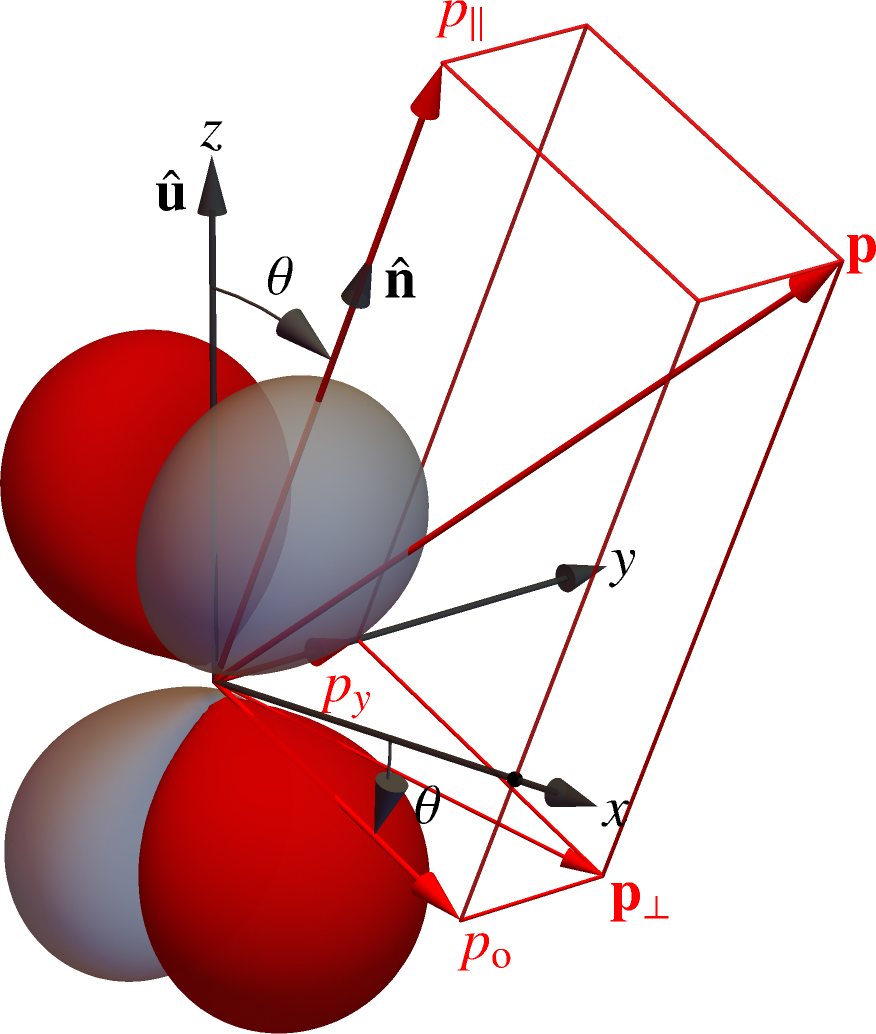
\includegraphics[scale=1]{2-ARM-theory/Figures/figure2F.png}
  \caption[Geometrical relationships between the molecular and the laser reference frames]{
  Geometrical relationships between the molecular and the laser (lab) frame. The $x$, $y$ and $z$ axis are on the molecular frame, with the internuclear axis $\uu$ along the $z$ axis. The laser polarization $\un$ is in the $x,z$ plane, with the momentum component $\pp$ along it; the transverse momentum vector $\vbpo$ has a component $\po$ in the molecular-laser ($x,z$) plane, and a shared component $p_y$ orthogonal to it.
  }
  \label{f2-molecular-frame}
\end{figure}



To tie this expression down a bit further, we introduce some additional notation to link together the molecular frame of reference with the laser, as shown in Figure~\ref{f2-molecular-frame}. We take $\un\cdot\uu=\cos(\theta)$ to give the angle $\theta$ between the internuclear axis and the laser polarization, and $\uu\cdot\vbpo=-\po\sin(\theta)$ as defining the transverse momentum component in the molecular-laser plane. With this notation, the leading-order shape factor reads
\begin{align}
\sft(\vbq)
& \approx
(-i)^n
\frac{e^{ \kappa a }}{\kappa a}
\frac{ v_x^{n_x}v_y^{\smash[b]{n_y}} v_z^{n_z}}{\kappa^{n_x+n_y+n_z}}
\cos\left(
b \left(
   \frac{\po}{\kappa}\sin(\theta)
   +i \left(1+\frac{\pt^2}{2\kappa^2}\right)\cos(\theta)
 \right)
\right)
%
\nonumber\\ & \quad   \times 
%
\left( 
1 
+ c\left(
  \frac{\po^2}{\kappa^2}\cos(2\theta)
  +\left(1+\frac{p_y^2}{\kappa^2}\right)\cos^2(\theta)
  -\frac{i}{2} \sqrt{1+\frac{\pt^2}{\kappa^2}}\frac{\po}{\kappa}\sin(2\theta)
\right)
\right)
.
\label{e2-leading-asymptotic-sft-molecular}
\end{align}


It is important to note, on the other hand, that the full analytical spherical Fourier transform $\sft(\vbq)$ as calculated in \eqref{e2-sft-final-analytical-result} does have some (unphysical) dependence on $a$, which is caused by the stack of approximations taken over the course of this chapter. This dependence disappears for large enough $\kappa a$, as shown in \reffig{f2-sft-asymptotics}, though in general this tends to happen for larger boundary radii than the equilibrium point between the laser and the Coulomb field. In practice, then, one needs to take the boundary radius $a$ at a point where the shape factor reproduces a shape consistent with the asymptotics, and is reasonably flat with respect to increases in this radius.



\newcommand{\figuretwoCkappa}{1}
\newcommand{\figuretwoCc}{1}
\newcommand{\figuretwoCb}{2.5}
\newcommand{\figuretwoCpo}{0}
\newcommand{\figuretwoCpy}{0}%
\begin{figure}[htb]
  \centering
  \begin{tabular}{cc}
  (a) $n_x=0$, $n_z=0$ &
  (b) $n_x=1$, $n_z=0$ \\[-2mm]
  \subfigure{
    \label{f2-sft-asymptotics-a}
    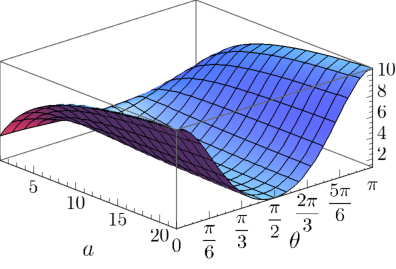
\includegraphics[scale=1]{2-ARM-theory/Figures/figure2Ca.pdf}
  }
  &
  \subfigure{
    \label{f2-sft-asymptotics-b}
    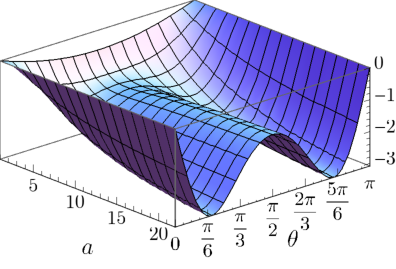
\includegraphics[scale=1]{2-ARM-theory/Figures/figure2Cb.pdf}
  }
  \\
  (c) $n_x=0$, $n_z=1$ &
  (d) $n_x=1$, $n_z=1$ \\[-2mm]
  \subfigure{
    \label{f2-sft-asymptotics-c}
    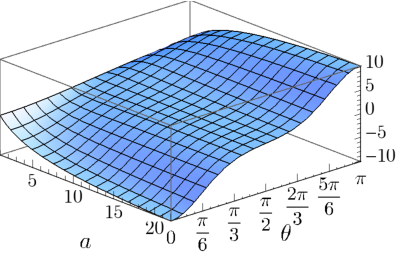
\includegraphics[scale=1]{2-ARM-theory/Figures/figure2Cc.pdf}
  }
  &
  \subfigure{
    \label{f2-sft-asymptotics-d}
    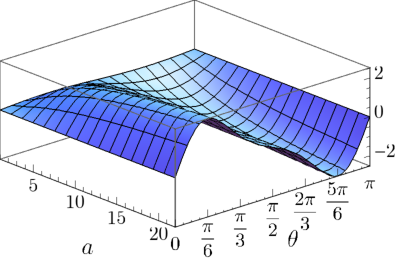
\includegraphics[scale=1]{2-ARM-theory/Figures/figure2Cd.pdf}
  }
  \end{tabular}
  \caption[Asymptotic behaviour of the spherical Fourier transform as a function of $a$]{
  Behaviour of the on-axis spherical Fourier transform, with the main asymptotic behaviour factored out as $\kappa a \:e^{-\kappa a}\:\sft(\vbq)$ and evaluated at the temporal saddle point at zero transverse momentum, as a function of the alignment angle $\theta$ and the boundary radius $a$, in the asymptotic region of the latter. 
  Here $\kappa=\figuretwoCkappa$, $c=\figuretwoCc$, $b=\figuretwoCb$, and $n_y=0$.}
  \label{f2-sft-asymptotics}
\end{figure}





Additionally, it is possible to go beyond the leading-order dependence of $\sft$ on $a$ and produce an asymptotic series for the limit $\kappa a \gg 1$ that produces better approximations to the shape factor (intermediate between the exact integral \eqref{e2-sft-final-analytical-result} and the leading asymptote \eqref{e2-leading-asymptotic-sft}) at moderate values of the boundary radius. Unfortunately, even to subleading order this produces rather unwieldy expressions, so they are omitted here for brevity, but they are implemented, and documented, in \citer{ARMSupport}.



More practically, the key feature of the molecular shape factor comes from its behaviour on axis: that is, for momenta very close to the laser polarization, at $\vbpo=0$, since it is harder for electrons to tunnel into nonzero transverse velocities. Thus, it is the on-axis shape factor $\left.\sft(\vbq) \right|_{\vbpo=0}$ that determines most of the effect of the electronic orbital in question and the molecule's orientation with respect to the laser field, along with its first-order dependence on $\vbpo$ at that point; we show both quantities in \reffig{f2-sft-on-axis}. 

Specifically, it is important to note that the main dependence, through $\left.\sft(\vbq) \right|_{\vbpo=0}$, will vanish when the alignment angle $\theta$ is such that the laser polarization lies along a node of the electronic orbital under consideration. In these conditions, ionization can proceed via direct ionization from other orbitals, but it can also do so via the correlation-driven mechanism which is derived below and which, as we will explore in chapter~\ref{chap:multi-channel}, relies crucially on the transverse momentum derivatives of the shape factor.





\newcommand{\figuretwoDkappa}{1.2}
\newcommand{\figuretwoDb}{2.5}
\newcommand{\figuretwoDc}{0.3}
\newcommand{\figuretwoDaone}{10}
\newcommand{\figuretwoDatwo}{50}%
\begin{figure}[htb]
  \centering
  \begin{tabular}{cc}
  (a) $n_x=0$, $n_z=0$ ($-\ \Sigma_g$) &
  (b) $n_x=1$, $n_z=0$ ($\B\ \Sigma_u$) \\[-2mm]
  \subfigure{
    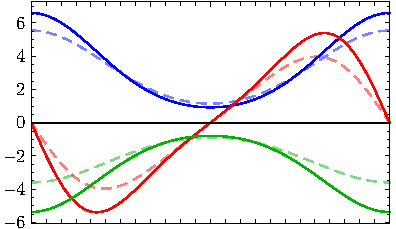
\includegraphics[scale=1]{2-ARM-theory/Figures/figure2Da.pdf}  
  }
  &
  \subfigure{
    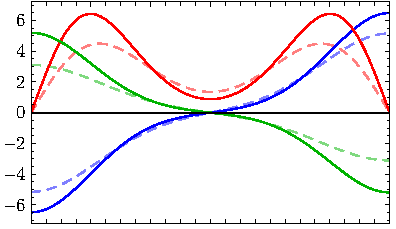
\includegraphics[scale=1]{2-ARM-theory/Figures/figure2Db.pdf}  
  }
  \\
  (c) $n_x=0$, $n_z=1$ ($\A\ \Pi_u$) &
  (d) $n_x=1$, $n_z=1$ ($\X\ \Pi_g$) \\[-2mm]
  \subfigure{
    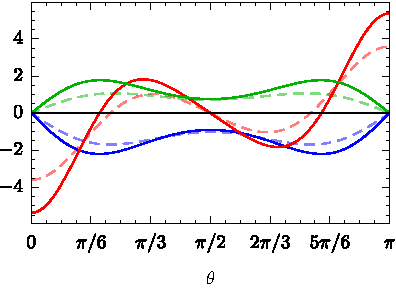
\includegraphics[scale=1]{2-ARM-theory/Figures/figure2Dc.pdf}  
  }
  &
  \subfigure{
    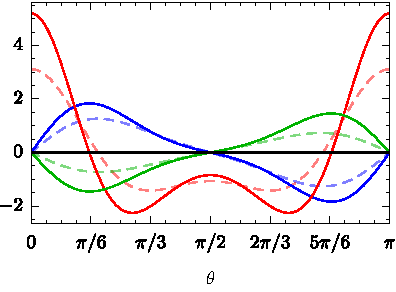
\includegraphics[scale=1]{2-ARM-theory/Figures/figure2Dd.pdf}  
  }
  \end{tabular}
  \caption[On-axis spherical Fourier transform, and its derivatives, as a function of molecular alignment angle]{Behaviour of the on-axis spherical Fourier transform $\left. \kappa a\: e^{-\kappa a}\:\sft(\vbq) \right|_{\vbpo=0}$ (blue) and its derivatives with respect to $\po$ (red) and $p_y$ (green), taken in the asymptotic region at $a=\figuretwoDatwo$. The regime of intermediate $a$, shown dashed at $a=\figuretwoDaone$, captures most of the qualitative behaviour but it is not quantitatively accurate.
  Here $\kappa=\figuretwoDkappa$, $c=\figuretwoDc$ and $b=\figuretwoDb$, corresponding to a reasonable model for the CO$_2$ molecule, and the different geometries are labelled by the orbital symmetry they produce and the corresponding states of the CO$_2$ molecule. We take $n_y=0$ for $\sft$, $\partial_\po\sft$, and the symmetry assignments, and $n_y=1$ for $\partial_{p_y}\sft$.
  }
  \label{f2-sft-on-axis}
\end{figure}








\section{Correlation-driven ionization}
\label{sec:correlation-driven-ionization}
We now turn to the correlation-driven ionization mechanism, which is embodied in the first-order term of the Dyson expansion of the wavefunction in powers of the correlation potential $V_{ee}^n$. We last saw this contribution in a split of the total wavefunction of the form $\ket{\Psi(t)}=\ket*{\Psi^{(0)}(t)}+\ket*{\Psi^{(1)}(t)}$ in \eqref{e2-decomposition}, in which the correlation-driven term had the form
\begin{align}
\ket{\Psi^{(1)}(t)}
=(-i)^2\sum_n  & \int\d\vb{k}\int^t\d t''\int^{t''}\d t'U^N(t,t'')V_{ee}^n(t'') U^{N-1}(t'',t')\ket{n(t')}
\nonumber \\ & \otimes 
U_e^n(t'',t')\ket{\vb{k}_n(t')}\times\matrixel{\vb{k}_n(t')}{\hat{L}^{(-)}(a)}{n_D(t')}e^{iI_p t'},
\label{e2-abstract-correlation-state-recall}
\end{align}
which we recall from \eqref{e2-abstract-correlation-state}.

The fist thing to do here is to tackle the full entangled propagator $U^N(t,t')$, which we tried to pretend was manageable by using the Dyson expansion to reduce it to a single separable propagator $U^{N-1}(t,t') \otimes U_e^n(t,t')$ but which, through the principle of conservation of hard work, is of course still present. And similarly to the first time around, to deal with this entangling propagator we will continue to pretend that it can be reduced to the unentangled dynamics, and that
\begin{equation}
U^N(t,t') \approx U^{N-1}(t,t') \otimes U_e^n(t,t')
\end{equation}
inside the integral of \eqref{e2-abstract-correlation-state-recall}. This time, however, we are no longer pushing the nontriviality away into another corner of the room: instead, we are making the definite assertion that the entangling interaction, the correlation potential $V_{ee}^n$, contributes essentially only to first order in the Dyson series, and that further interactions are negligible.

We therefore make this key physical approximation, to get the correlation-driven contribution as
\begin{align}
\ket{\Psi^{(1)}(t)}
=(-i)^2\sum_n  & \int\d\vb{k}\int^t\d t''\int^{t''}\d t'U^{N-1}(t,t'') \otimes U_e^n(t,t'')V_{ee}^n(t'') U^{N-1}(t'',t')\ket{n(t')}
\nonumber \\ & \otimes 
U_e^n(t'',t')\ket{\vb{k}_n(t')}\times\matrixel{\vb{k}_n(t')}{\hat{L}^{(-)}(a)}{n_D(t')}e^{iI_p t'},
\label{e2-abstract-correlation-state-approximate}
\end{align}
and now we can begin simplifying this using many of the techniques we used for the direct ionization channel. Thus, analogously to our definition in \eqref{e2-ionization-yield} of the ionization yield, we have the correlation-driven yield given by
\begin{align}
a_n^{(1)}(\vb{p},& \tn)
=
\bra{\vb{p}}\otimes\bra{n(\tn)}U^{N-1}(\tn,T)\ket{\Psi^{(1)}(T)}
\nonumber \\ & =
(-i)^2\sum_m  \int\!\d\vb{k}\int^T\!\!\d t''\int^{t''}\!\!\!\!\d t'
\bra{n(\tn)}U^{N-1}(\tn,t'') \otimes \bra{\vb{p}}U_e^m(T,t'')
\times V_{ee}^m(t'') 
\nonumber \\ & \quad \quad \times
U^{N-1}(t'',t')\ket{m(t')}
\otimes 
U_e^m(t'',t')\ket{\vb{k}_m(t')}
\times\matrixel{\vb{k}_m(t')}{\hat{L}^{(-)}(a)}{m_D(t')}e^{iI_p t'}.
\label{e2-correlation-driven-yield-initial}
\end{align}

Here, similarly to the direct case in \eqref{e2-propagated-quasistatic-eigenstates}, we neglect the Stark shifting and field-induced transitions between the ionic eigenstates, so the ionic states propagate as the field-free $U^{N-1}(t'',t')\ket{n(t')}=e^{-iE_n(t''-t')}\ket{n}$, and we propagate the continuum states using \eqref{e2-channel-specific-eikonal-tdse}. This leaves us, then, with a much simpler expression:
\begin{align}
a_n^{(1)}(\vb{p},\tn)
& =
(-i)^2\sum_m  \int\!\d\vb{k}\int^T\!\!\d t''\int^{t''}\!\!\!\!\d t'
e^{+iE_n(t''-\tn)}
e^{-iE_m(t''-t')}
\nonumber \\ & \qquad \quad
\times
\bra{n} \otimes \bra{\vb{p}_n(t'')}
V_{ee}^m
\ket{m}
\otimes 
\ket{\vb{k}_m(t'')}
\times\matrixel{\vb{k}_m(t')}{\hat{L}^{(-)}(a)}{m_D}e^{iI_p t'}.
\label{e2-correlation-driven-yield-second}
\end{align}

In fact, this expression separates completely into an ionization part, with a temporal integral over $t'$ -- which we term the ionization time -- and a temporal integral over $t''$, which we term the interaction time, giving
\begin{align}
a_n^{(1)}(\vb{p},\tn)
& =
-i 
e^{-iE_n \tn}
\sum_m  \int\!\d\vb{k}   \int^T\!\!\d t''
e^{+i(E_n-E_m)t''}
\bra{n} \otimes \bra{\vb{p}_n(t'')}
V_{ee}^m
\ket{m}
\otimes 
\ket{\vb{k}_m(t'')}
\nonumber \\ & \qquad \qquad \quad  \times
(-i)\int^{t''}\!\!\d t'
e^{+iE_m t'}
\matrixel{\vb{k}_m(t')}{\hat{L}^{(-)}(a)}{m_D}e^{iI_{p,m} t'}.
\label{e2-correlation-driven-yield-separated}
\end{align}
Moreover, the internal integral over the ionization time $t'$ is exactly of the same form as the direct ionization amplitude \eqref{e2-sae-yield-beginning}, with the only difference being that the upper limit, $t''$, is now variable and potentially complex, so we can directly apply the results from the previous development. The second line of \eqref{e2-correlation-driven-yield-separated} is therefore exactly equal to $e^{+iE_mt''}a_m^{(0)}(\vbk,t'')$, and it can be replaced with the final result from \eqref{e2-ionization-yield-with-shape-factor} to give
\begin{align}
a_n^{(1)}(\vb{p},\tn)
& =
-i 
e^{-iE_n \tn}
\sum_m  \int\!\d\vb{k}   \int\!\d t''
e^{+i(E_n-E_m)t''}
\bra{n} \otimes \bra{\vb{p}_n(t'')}
V_{ee}^m
\ket{m}
\otimes 
\ket{\vb{k}_m(t'')}
\nonumber \\ & \qquad \qquad \quad  \times
e^{iI_{p,m} \ts - \frac{i}{2} \int_{\ts}^{T}\left(\vbk+\vba(\tau)\right)^2\d\tau }
e^{-i\int_\tk^{t''} U_m\left(\int_{ \ts}^\tau \vbk+\vba(\tau')\d\tau'\right) \d\tau}
R_m(\vbk)
.
\label{e2-correlation-driven-yield-with-a1-included}
\end{align}

This expression admits a simple interpretation, with the electron being ionized at the complex time $\ts$ into a superposition of channels $\ket{m}$ and intermediate momenta $\vbk$, and then subsequently interacts with the ion at time $t''$ to get to its final channel $n$ and momentum $\vbp$. As far as the continuum electron is concerned, then, the main part of the interaction is the single-electron operator
\begin{equation}
\matrixel{n}{V_{ee}^m}{m}
=
\matrixel**{n}{\left(\vphantom{\sum}V_{ee}-\bra{n}V_{ee}\ket{n}\right)}{m}.
\end{equation}
This operator must be handled in the position representation, since the electrostatic interaction is defined as such by definition \eqref{e2-V-ee-definition}. We therefore encase it inside position eigenstates to get a single function of position,
\begin{equation}
\matrixel**{\vbr'}{
\vphantom{\sum}
\matrixel{n}{V_{ee}^m}{m}
}{\vbr}
=
\bra{\vbr'}\otimes\bra{n}
{\left(\vphantom{\sum}V_{ee}-\bra{n}V_{ee}\ket{n}\right)}
\ket{\vbr}\otimes\ket{m}
\equalscolon
\delta(\vbr-\vbr')
\Vnm{\vbr},
\label{e2-Vnm-definition}
\end{equation}
which we encapsulate in the shorthand notation $\Vnm{\vbr}$.

Doing the matrix element of \eqref{e2-correlation-driven-yield-with-a1-included} in the position representation, then, leaves us with the expression
\begin{align}
a_n^{(1)}(\vb{p},\tn)
& =
-i 
e^{-iE_n \tn}
\sum_m  \int\!\d\vbk   \int\!\d\vbr  \int\!\d t''
e^{+i(E_n-E_m)t''}
\Vnm{\vbr}
\braket{\vb{p}_n(t'')}{\vbr}
\braket{\vbr}{\vb{k}_m(t'')}
\nonumber \\ & \qquad \qquad \quad  \times
e^{iI_{p,m} \ts - \frac{i}{2} \int_{\ts}^{T}\left(\vbk+\vba(\tau)\right)^2\d\tau }
e^{-i\int_\tk^{t''} U_m\left(\int_{ \ts}^\tau \vbk+\vba(\tau')\d\tau'\right) \d\tau}
R_m(\vbk)
.
\label{e2-correlation-driven-yield-position-representation}
\end{align}
Here we use the explicit form of the eikonal Volkov states, \eqref{e2-eikonal-volkov-wavefunctions}, to further pin down this ionization yield into the explicit form
\begin{align}
a_n^{(1)}(\vb{p},\tn)
& =
-i 
\sum_m 
e^{-iE_n \tn}
e^{iI_{p,m} \ts}
\int\!\d t''
e^{+i(E_n-E_m)t''}
e^{-\frac{i}{2} \int_{t''}^T\left(\vbp+\vba(\tau)\right)^2\d\tau} 
\nonumber \\ & \quad \ \  \times
\frac{1}{(2\pi)^{3}}
\int\!\d\vbk
\int\!\d\vbr \:
\Vnm{\vbr}
R_m(\vbk)
e^{i\left(\vbk-\vbp\right)\cdot\vb{r}} 
e^{-\frac{i}{2} \int_{\ts}^{t''}\left(\vb{k}+\vba(\tau)\right)^2\d\tau} 
e^{-iW_{nm}(\vbr,\vbk,t'')}
,
\label{e2-correlation-driven-yield-with-eva-states}
\end{align}
where the Coulomb correction now reads
\begin{align}
W_{nm}(\vbr,\vbk,t'')
& =
-\int_{t''}^T U_m(\rl(\tau;\vb{r},\vb{k},t''))\d\tau
-\int_\tk^{t''} U_m\left(\rl(\tau;\vb{0},\vb{k},t'')\right) \d\tau
\nonumber \\ & \qquad +
\int_{t''}^T U_n(\rl(\tau;\vb{r},\vbp,t''))\d\tau
.
\label{e2-correlation-channel-coulomb-correction}
\end{align}


Finally, we address the limits for the interaction-time integration over $t''$, which originally went from $-\infty$ to the large detection time $T$. However, the $t'$ integral in \eqref{e2-correlation-driven-yield-separated} only went up to $t''$, and this means that for the direct-channel result to hold we need the integration range over $t''$ to be restricted to times after the ionization event $\ts$ to which we've collapsed the entire $t'$ integral. This means, then, that the correlation-driven yield can be written down as
\begin{align}
a_n^{(1)}(\vb{p},\tn)
& =
-i 
\sum_m 
e^{-iE_n \tn}
e^{iI_{p,m} \ts}
\int_{\ts}^T\!\d t''
e^{+i(E_n-E_m)t''}
e^{-\frac{i}{2} \int_{t''}^T\left(\vbp+\vba(\tau)\right)^2\d\tau} 
\nonumber \\ & \quad \ \  \times
\frac{1}{(2\pi)^{3}}
\int\!\d\vbk
\int\!\d\vbr \:
\Vnm{\vbr}
R_m(\vbk)
e^{i\left(\vbk-\vbp\right)\cdot\vb{r}} 
e^{-\frac{i}{2} \int_{\ts}^{t''}\left(\vb{k}+\vba(\tau)\right)^2\d\tau} 
e^{-iW_{nm}(\vbr,\vbk,t'')}
.
\label{e2-correlation-driven-yield-semi-final}
\end{align}
This form for $a_n^{(1)}(\vb{p},\tn)$ is now essentially ready -- or, at least, it cannot be processed much further without more knowledge about the system in question. (Here the Coulomb correction \eqref{e2-correlation-channel-coulomb-correction} can use further simplification, but we will not discuss it further and we will make the reasonable approximation that its behaviour will be similar to the correction in the direct case.) 

There are two main parts of this expression, and they fulfil two different roles. On one side there is the spatial description, which involves the integrals over $\vbr$ and $\vbk$, which determines how the geometry of both channels influences the behaviour of the correlation-driven channel, and this will be the main focus of the following chapter.

Overarching this geometrical dependence, however, is a more fundamental dynamical statement about the behaviour of this correlation-driven tunnelling, coming from the temporal integral over $t''$ and its various factors. This integral is not trivial, because in shifting the $t'$ integral to its complex saddle point $\ts$, we have also brought the starting point of the interaction-time integral over $t''$ to a complex time. Since here, as before, $t''$ appears in exponential factors of the form $e^{iEt''}$, the imaginary part of $t''$ plays a crucial~role.

At heart, the temporal dependence in \eqref{e2-correlation-driven-yield-semi-final} contains a conflict between two colliding factors that try to pull the main contributions to the integral to different regions of $t''$, and the resolution of this conflict is a compromise that makes much of the interaction happen inside the tunnelling barrier.

On one side of this conflict is the exponential factor $e^{+i(E_n-E_m)t''}$, which is a phase for real $t''$ but can provide large amplitude changes for the regions where it is complex. In general, this factor will tend to aid ionization into excited states ionic by letting the electron ionize from the highest-lying occupied orbital, which is easier to tunnel from, and then change channels once they've gone through much of the tunnelling barrier. In this case, the initial channel $m$ is the ground ionic state, and the final channel $n$ has a higher energy, so~that
\begin{equation}
\Delta I_{p,nm}=E_n-E_m
\end{equation}
is a positive quantity. In this regime, the amplitude of the exponential factor is given by
\begin{equation}
\left|e^{+i(E_n-E_m)t''}\right|
=
e^{-\Delta I_{p,nm}\Im(t'')},
\end{equation}
where in general $\Im(t'')$ will be between 0 and $\Im(\ts)>0$. This exponential dependence will tend to select interaction times with smaller imaginary parts, relatively far away from the ionization time $\ts$, and therefore as far into the barrier as possible.


On the other side of this conflict is the spatial dependence, more specifically through the decay of the interaction potential $\Vnm{\vbr}$ at larger distances. As we shall see in chapter~\ref{chap:multi-channel}, a saddle-point argument on the geometrical integrals over $\vbk$ and $\vbr$, driven by the exponential factors $\exp\left(i\left( \vbk- \vbp\right) \cdot\vb{r}-\frac{i}{2} \int_{\ts}^{t''} \left(\vb{k} + \vba(\tau) \right)^2\d\tau\right)$ of \eqref{e2-correlation-driven-yield-semi-final}, indicates that the contributions to spatial integral are mostly concentrated in a region around the laser-driven trajectory $\rl(t'') = \int_{\ts}^{t''} \vbp+\vba(\tau)\d\tau$, and this will tend to go away from the origin (and rather quickly so) as $t''$ goes from the ionization time $\ts$ towards its real part. Evaluated at this position, $\Vnm{\rl(t'')}$ will decrease in the same direction that the exponential factor is increasing. 

Taken together, both factors will make most of the interaction come from complex interaction times at which the electron is still in the mid-barrier regime, which makes the study of the interaction all the more interesting. In the following chapter we turn, therefore, to the study of the geometrical effects of this interaction, in the hopes of finding signatures that will help us show that these mid-barrier interactions are in fact occurring.































